\documentclass[12pt]{article}
\usepackage{graphicx}
\usepackage{graphics}
\usepackage[percent]{overpic}
\usepackage{hyperref}
\usepackage{indentfirst}
%\usepackage{setspace}
\renewcommand\theequation{{\color{red}\arabic{equation}}}
\hypersetup{colorlinks=true}
\usepackage{amsmath}
\usepackage{empheq}
\usepackage{amsfonts}
\usepackage{float}
\usepackage{algorithm}
\usepackage{algorithmic}
\usepackage{caption}
\usepackage{subfigure}
%\usepackage{subcaption}
\usepackage[numbers]{natbib}
\usepackage{lipsum}
\bibliographystyle{plainnat}%{ieeetr}%Choose a bibliograhpic style
\usepackage[toc,page]{appendix}
\addtolength{\textwidth}{1.1in}
\addtolength{\hoffset}{-0.5in}
\addtolength{\textheight}{1.1in}
\addtolength{\voffset}{-0.8in}
\usepackage{tikz,pgfplots}
\usetikzlibrary{arrows,snakes,backgrounds,spy,mindmap,trees}
\usetikzlibrary{er}
%\usepackage{onimage}
\pgfplotsset{compat=newest}
%\usepackage{setspace}
%\doublespacing
%\usepackage{parskip}
%\parskip=2\baselineskip \advance\parskip by 0pt plus 2pt 
\usepackage{rotating}
\newcommand{\mgnote}[1]{\textcolor{magenta}{MG: #1}}
\newcommand{\gsnote}[1]{\textcolor{blue}{GS: #1}}
\newcommand{\vrnote}[1]{\textcolor{red}{VR: #1}}
\newcommand{\IIinv}{{\dot\varepsilon}_{\mathrm{\!\!\:II}}}

\newcommand{\mm}{{\ensuremath{\boldsymbol{m}}}}
\newcommand{\uu}{{\ensuremath{\boldsymbol{u}}}}
\newcommand{\vv}{{\ensuremath{\boldsymbol{v}}}}
\newcommand{\ww}{{\ensuremath{\boldsymbol{w}}}}
\newcommand{\uobs}{{\ensuremath{\boldsymbol{u}_\text{obs}}}}
\newcommand{\ff}{{\ensuremath{\boldsymbol{f}}}}
\newcommand{\FF}{{\ensuremath{\boldsymbol{F}}}}
\newcommand{\ppi}{{\ensuremath{\boldsymbol{\pi}}}}

\newcommand{\ssigma}{{\ensuremath{\boldsymbol{\sigma}}}}
\newcommand{\strain}{{\ensuremath{\dot{\boldsymbol{\varepsilon}}}}}


%\let\oldabstract\abstract
%\let\oldendabstract\endabstract
%\makeatletter
%\renewenvironment{abstract}
%{\renewenvironment{quotation}%
%               {\list{}{\addtolength{\leftmargin}{1em} % change this value to add or remove length to the the default
%                        \listparindent 1.5em%
%                        \itemindent    \listparindent%
%                        \rightmargin   \leftmargin%
%                        \parsep        \z@ \@plus\p@}%
%                \item\relax}%
%               {\endlist}%
%\oldabstract}
%{\oldendabstract}
%\makeatother




\date{}

\title{Chapter 4: Inference of plate boundary properties with an adjoint optimization with large scale two-dimensional models}


\begin{document}
\maketitle
\begin{abstract}
 Plate motions are the primary surface observables available to constrain forward models and have been able to constrain the rheological properties of the mantle. While plate motion data is an important surface observation, there exist additional observations such as surface normal stresses and in some locations in the mantle, average effective viscosity, which arise from post-glacial rebound and earthquakes. While incorporating different pieces of data can provide refined estimates of the rheological parameters; however, there have been no estimates on the uncertainty of the stresses of plate boundaries, which has important consequences of where great earthquakes occur.  To this end, we will incorporate both plate motions and effective viscosity into our optimization framework and therefore derive the adjiont system and gradients for the inferred parameters. Furthermore, we will derive the posterior distributions for the normal and shear stresses within each plate boundary by making use of a Gaussian approximation which provides a first-order appoximation to the true posterior distribution. We will apply these new methods (average effective viscosity data and covariance estimates of the stresses) to various 2-D cross-sections of subduction zones, where we have a realistic temperature distribution and realistic fault zones from Slabs 1.0. From these models, we will analyze the conditional and marginal distributions and ascertain the correlations between the shear and normal stresses with the inferred rheological parameters such as the strain rate exponent and yield stress.
\end{abstract} 


\section*{Introduction}
While slab pull may be the dominant force driving plate motions and associated mantle flow, there remains substantial uncertainty on the relative coupling of stresses across plate boundaries at subduction zones. This coupling can either be attributed to broad-scale tectonics forces or to the varying properties between the plates at each subduction zone. While it is not clear whether broad-scale forces or the varying tectonic properties have the stronger contribution to the variations in seismic coupling, a valid model should appropriately represent the broad-scale forces. 
Seismic coupling is defined as the ratio between the observed seismic moment release to the rate of plate tectonic velocities and generally varies between 0 and 1. Seismic coupling is sensitive to the short window of recorded earthquakes such that if many large magnitude earthquakes occur within that short window then the seismic coupling could be close to or even exceed unity, whereas if no large magnitude earthquakes occur, then the seismic coupling will be small.  While seismic coupling is a reasonable way to build a relationship to forecast which subduction zones have a propensity for future large magnitude events, other pieces of data such as the curvature of subduction zones can be used to determine where great earthquakes are more likely to occur \citep{bletery2016mega}. 

  %It was suggested in \citep{ide2013proportionality} that background seismicity can be correlated with subduction zones that have experienced great earthquakes. %Additionally, there might be a correlation between the plate age and b-value \citep{nishikawa2014earthquake}. These results lead to relating the shear and normal stresses (broad-scale forces) at plate boundaries to background seismicity and b-values in addition to the geodetic seismic coupling.

Regardless of whether broad-scale forces or varying shear zone properties are the ultimate cause for variations in seismic coupling, geodynamic models should be able to explain variations between the two endmembers from the least coupled Marianas subduction zone and the most coupled Chilean. The Chilean subduction zone is among the most seismically active with many earthquakes above 8, including the largest ever recorded , the 1965 Valdivia earthquake with magnitude 9.5. Chile, overall is in a state of compression on the South American margin, on the other hand the Marianas subduction is among the least seismically coupled with no historic earthquake greater than. Morevoer, the Marians subduction zone is characterized by active back arc openig within the Marianas Trough.


A simple force balance of subduction zones that parameterize the broad-scale forces heuristically suggests a link between tectonic forces and how seismically coupled subduction zones are \citep{scholz1995mechanism, scholz2012seismic}. Those models analyze subduction zones  case by case where where the force distribution arises from slab pull and an anchoring force. Furthermore, those models do not include key variantions in rheology and how it would influence the distribution of  normal forces.  While that study found a relationship between broad-scale forces and coupling, their approach was simple and may not capture the essence of the system as the actual geometry of slabs is complex with complex flow patterns induced by global flow \citep{scholz2012seismic}. The simple models seem to incorrectly capture how buoyancy forces and the resulting flow interact.

%The partitioning of the resisting forces can be seen through the plate-coupling of the weakzone factors in the rheological relationship, which provides the effective frictional resistance in models. There have been investigations into these ideas and how different subduction zones have different fricitional forces.  The notion of coupling can be either mechanical or tectonic coupling. Both ideas can lead to the end member cases 

  To accurately estimate the forces at plate boundaries, not only is the correct physics needed, but any optimization scheme must be constrained by observed plate motion \citep{BursteddeStadlerAlisicEtAl13,Stadler27082010} the most robust constraint on mantle flow. We overcome these limitations by employing a method similar to our earlier work \citep{ratnaswamy2015adjoint} where we use rigid plate data on areas away from deforming plate boundaries essentially allowing for self-consistent deformation within plate boundaries. Furthermore, the shape of the fault zones play a key role in governing plate motions \citep{Zhong10021995}, but these can be mapped at shallow depths with seismic observations and need to be incorporated as constraints \citep{Hayes2012}.
Augmenting the surface velocity data, we now incorporate constraints on the average of viscosity within selected regions. Estimates of the average effective viscosity constraints arise from post-glacial rebound and earthquakes.  Using constraints on viscosity allows for a better estimation of the strain rate exponent, upper mantle prefactor or any bulk effective mantle properties compared to solely using plate motion data. 

In addition to incoporating the average effective viscosity as data, we recognize the need to estimate the shear and normal stresses at plate boundaries. We can estimate the cumulative stresses after an optimization, however, the tradeoffs between the calculated stresses and inferred rheological parameters is unknown. 

 In this chapter, we will not only explore the incorporation of average effective viscosities, but within the optimization, estimate uncertainties of stresses (in both a normal and shear sense) in fault zones. While inferring plate boundary strength factors \citep{ratnaswamy2015adjoint} can lead to a better understanding of which plate boundaries are more mechanically coupled, such variables do not have physical units and so here we not only estimate the magnitude of  stresses but also their uncertainties. We will derive expressions for the gradients of inferred parameters using average effective viscosity. Furthermore, we will derive expressions for the covariance matrices of the average normal and shear stresses (under the assumption that model noise follows a Gaussian distribution). We will then apply these methods to a 2D cross-sectional slice with observed plate motions and viscosity constraints, but with thermal structures and fault zone geometries constrained by a variety of other (primarily seismic) data.
 


\section*{Methods}
We will build upon our earlier work \citep{ratnaswamy2015adjoint} by adding several fundamental enhancements. We recognize the need to quantify the uncertainty of the plate boundary stresses since the uncertainty and correlations of the stress with each rheological parameter gives a more meaningful physical interpretation of the interplay between stresses and rheology. However, the stresses in the fault zones are not initially (directly) inferred with our adjoint formulation, and thus do not have a covariance distribution readily available. A Markov Chain Monte Carlo (MCMC) approach would likely recover the covariance but would require many samples (forward solutions) and make the optimization computationally intractable. Alternatively, we will derive Gaussian approximations for the covariance distributions for the stresses within fault zones.
 Additionally, we will incorporate the average effective viscosity for selected regions in the mantle where such constraints exist. 
The average effective viscosity and plate velocities will provide a better estimate for the rheological parameters which in turn lead to refined estimates on the stresses within plate boundaries. Incorporating the average effective viscosity requires the derivation of a new adjoint system that will be developed here. 

Using the same method as in \citep{ratnaswamy2015adjoint}, we only use observations within the rigid parts of the plate (middle 80$\%$) so as to avoid the plate boundaries and respect the deformation that occurs at plate boundaries. 


\subsection*{Stress}
Earlier (Chapter 2), we inferred global parameters in the rheological relationship for the mantle with an adjoint optimization which the viscosity is defined as,
  \begin{equation}
    \eta(\IIinv,\sigma_{y}) =
\eta_{\min} + \min(\Gamma_i\min(\eta_{\max},a(T)(\IIinv-d)^{\frac{1}{2n}}\IIinv^{-\frac{1}{2}}),
\frac{1}{2}\sigma_y\IIinv^{-\frac{1}{2}})
\label{eq:rheo}
  \end{equation}
where $\eta_{min}$ is the minimum effective viscosity, $\sigma_y$ is the yield stress, $a(T)$ is the temperature dependent component of viscosity, $n$ is the strain rate exponent and $d$ is a parameter included to regularize the solution. While some of the parameters, weakfactor $\Gamma$, do not have physical units and arise in the geophysical problem, the parameters  $n$ and $\sigma_y$ can at least be partially inferred from laboratory experiments\citep{korenaga2008new}. In the earlier models we were able to estimate the parameters in the rheological relationship for synthetic models; however, there were no bounds placed on the uncertainty of derived quantities that are dependent on the rheological parameters, such as the shear stresses \citep{ratnaswamy2015adjoint}. %Furthermore, the relationship between the stress (normal and tangential) and the global rheological parameters is not known. 

 Here, we must build an approximation of derived quantities, especially the stress. This quantity is embedded in the weakfactors, but the weakfactors are a parameterization, so we need to map those to stresses.
There are multiple measures of stress in a weakzone (normal, tangential) as well as the square-root of the second invariant of the stress tensor ($\sigma_{avg}$), i.e. 
\begin{equation}
\sigma_{avg} = \int_{\Omega_w} (\ssigma:\ssigma)^{\frac{1}{2}} d\Omega_i
\end{equation}
Helpful quantities for addressing the origin of seismic coupling through the geographic variability of great earthquakes, include the average shear ($\sigma^t_{avg}$) and normal tractions ($\sigma^n_{avg})$ in the weakzones,
\begin{equation}
\sigma^n_{avg} = \int \textbf N \sigma\cdot\textbf n d\Omega_w
\end{equation}

\begin{equation}
\sigma^t_{avg} = \int \textbf T \sigma\cdot\textbf n d\Omega_w
\label{eq:normal_traction}.\
\end{equation}
The normal and shear components of the stress are more importatnt than the second invariant of the stress tensor as they effectively give the resisting stresses along the plate boundaries. The larger the resisting stress, the more coupled a plate boundary, and vice versa. Here, \textbf{T} and \textbf N are the tangential and normal projection along the center line of the plate boundaries,
\begin{equation}
\begin{split}
        \textbf T = \textbf I -\text n_w \otimes \text n_w\\
        \textbf N = \text n_w \otimes \text n_w\\
\end{split}
\end{equation}

 We know that we estimate the Gaussian distribution of the weak factors, i.e.,

\begin{equation}
\ppi_{\Gamma_i} = \mathcal N(\Gamma_i^{map}, \sigma_{\Gamma_i})
\end{equation}
However, we also are interested in the stresses in each plate boundary, 
\begin{equation}
\ppi_{\sigma^n_i} = \mathcal N(\sigma_i^{map}, \sigma_{\sigma_i})
\end{equation}
because they give a more natural interpretation of plate coupling as opposed to the weakfactor parameterization ($\Gamma_i$).
Starting with the normal distribution,
\begin{equation}
\mathcal N(\mu_{map},\sigma) = \int\frac{1}{\sigma\sqrt{2\pi}}\exp({-\frac{(x-\mu_{map})^2}{2\sigma^2}})dx
\end{equation}

As we do not infer the shear or normal stresses, we instead build the Gaussian approximation to the normal stress. A natural question would be how well the shear and normal stresses are approximated by a Gaussian distribution. Locally, near the \textbf{MAP} point, the conditional stresses and to an extent the marginal distributions are well approximated by a Gaussian distribution \citep{ratnaswamy2015adjoint}.  We define a measure of the stress from the underlying properties such as the strain rate exponent, yield stress and so forth, e.g. $\mm$ as, 
\begin{equation}
\textit \ssigma = f(\mm)
\end{equation}
expanding $\ssigma$,
\begin{equation}
\ssigma (\mm) = \ssigma(\mm_{map}) + \frac{\partial\ssigma}{\partial \mm}|_{\mm_{map}} (\mm-\mm_{MAP}) + h.o.t
\end{equation}
The mean of \ssigma is $\ssigma(\mm_{map})$, while the covariance is defined as,
\begin{equation}
\mathcal C = \mathcal E[(\ssigma-\mu_{\ssigma})^T(\ssigma-\mu_{\ssigma})]
\end{equation}
or, 
\begin{equation}
\mathcal C = \mathcal E[(\ssigma-\ssigma(\mm_{map}))^T(\ssigma-\ssigma(\mm_{map}))]
\end{equation}
where $\mathcal E$ denotes the expectation (i.e. the mean). For example, the expected value of a continuous random variable $x$ is defined,
\begin{equation}
\mathcal E(x):= \int x p(x) dx
\end{equation}
where $p(x)$ is the probability distribution of $x$.
The expected value of a normal distribution $\mathcal{N}(\mu_{MAP},\sigma^2)$ is,
\begin{equation}
\mathcal E(x):= \int x \frac{1}{\sigma\sqrt{2\pi}}\exp({-\frac{(x-\mu_{map})^2}{2\sigma^2}}) dx = \mu .\
\end{equation}
Using a Taylor series expansion of the  stress, while only retaining the $1^{st}$ order terms, we obtain
\begin{equation}
\ssigma (\mm) -\ssigma(\mm_{map}) \approx \frac{\partial\ssigma}{\partial \mm} (\mm-\mm_{MAP})
\end{equation}
Therefore
\begin{equation}
\mathcal C = \mathcal E\big[\big(\frac{\partial\ssigma}{\partial \mm}|_{\mm_{map}} (\mm-\mm_{MAP})\big)^T\big(\frac{\partial\ssigma}{\partial \mm}|_{\mm_{map}} (\mm-\mm_{MAP})\big)\big]
\end{equation}
which leads to
\begin{equation}
\mathcal C = \big(\frac{\partial\ssigma}{\partial \mm}|_{\mm_{map}}^T \mathcal E[(\mm-\mm_{MAP})^T(\mm-\mm_{MAP})](\frac{\partial\ssigma}{\partial \mm}|_{\mm_{map}}\big)
\end{equation}
where 
\begin{equation}
  \mathcal E[(\mm-\mm_{MAP})^T(\mm-\mm_{MAP})] = \mathcal H^{-1}(\mm) = \mathcal C(\mm)
  \end{equation}
leading to
\begin{equation}
\mathcal C(\ssigma) = \frac{\partial\ssigma}{\partial \mm}|_{\mm_{map}}^T \mathcal H^{-1}(\mm)\frac{\partial\ssigma}{\partial \mm}|_{\mm_{map}}
\end{equation}
or 
\begin{equation}
\mathcal C(\ssigma) = \frac{\partial\ssigma}{\partial \mm}|_{\mm_{map}}^T \mathcal C(\mm)\frac{\partial\ssigma}{\partial \mm}|_{\mm_{map}}
\end{equation}
with $\mathcal C(\mm)$ is the covariance matrix obtained from solving for the MAP point in the original optimization problem. Therefore, the normal distribution of the stresses is
\begin{equation}
  \ppi_{\ssigma} = \mathcal N\big(\ssigma(\mm_{map}), \frac{\partial\ssigma}{\partial \mm}|_{\mm_{map}}^T \mathcal C(\mm)\frac{\partial\ssigma}{\partial \mm}|_{\mm_{map}}\big)
\end{equation}

%\section*{RHS of adjoint solve}
To form the Gaussian approximation of the stress within each weakzone, we compute the gradient of the stress with respect to the inferred parameters. This amounts to solving an adjoint solve, and a gradient computation. Taking variations of ~\eqref{eq:normal_traction} with respect to the velocity,
\begin{equation}
\sigma^t_{avg}=\textbf{T}\cdot\frac{\partial\sigma}{\partial \textbf u}\cdot \textbf n
\end{equation}
with,
\begin{equation}
\frac{\partial\sigma}{\partial \textbf u} = \frac{\partial \eta}{\partial \textbf u}\overset{.}{\epsilon}(\textbf u)
                                            + \eta\overset{.}{\epsilon}(\delta \textbf u)
\end{equation}
This is just an application of the linearized Newton operator to the velocity of the forward model at the \textbf{MAP} point.
For the second invariant of the stress tensor, one will have extra terms compared to the average stress,
\begin{equation}
  \begin{split}
 \ssigma_{II}& = \frac{1}{2}\textbf{Tra}(\ssigma:\ssigma) \\
 & = \frac{1}{2}[\eta\strain(\uu):\eta\strain(\uu)]\\
             & = \frac{1}{2}[\strain(\uu):\eta^2\strain(\uu)]
\end{split}
\end{equation}
then,
\begin{equation}
    \frac{\partial \ssigma_{II}}{\partial \uu} = \strain(\delta \uu):\eta^2\strain(\uu) +
 \strain(\uu):\strain(\uu)\eta\frac{\partial\eta}{\partial \IIinv}(\strain(\uu):\strain(\delta\uu)
\end{equation}
%\section*{Computing the Gradient after the adjoint solve}
After solving for the adjoint solution above, we then compute the gradient for ~\eqref{eq:normal_traction},
\begin{equation}
\mathcal{G}:=  \textbf{T}\frac{\partial{\ssigma}}{{\partial \mm}}\cdot \textbf{n}
\end{equation}
where,
\begin{equation}
\frac{\partial \ssigma}{\partial \mm} = \eta_{,i}\strain(\uu)
\end{equation}
For the second invariant of the stress tensor, 
\begin{equation}
\mathcal G:=  \strain(\uu):2\eta\cdot\eta_{,\mm}\strain(\uu)
\end{equation}

\begin{align*}
  &\eta_{,i}(\IIinv,\Gamma,n,\sigma_y) \\
  &\quad=\begin{cases}
    0 & \text{ in } \Omega_y,\\
    \Gamma_i\chi_i\min(\eta_{\max},a(T)(\IIinv-d)^{\frac{1}{2n}}\IIinv^{-\frac{1}{2}})
    & \text{ in } \Omega\setminus\Omega_y.
  \end{cases}
\end{align*}
where $\Gamma_i = \exp(m_i)$.
\begin{equation*}
  \eta_{,i}(\IIinv,\Gamma,n,\sigma_y) =
  \begin{cases}
    \frac{1}{2}\sigma_y\IIinv^{-\frac{1}{2}} & \text{ in } \Omega_y,\\
    0                          & \text{ in } \Omega\setminus\Omega_y.
  \end{cases}
  \end{equation*}
%\vrnote{the above does not need a $\min$ because $\sigma_y >0$ and $\IIinv$ is non-negative}
Finally, if $m_i = \log(n)$, we obtain
\begin{align*}
  \eta_{,i}(\IIinv,\Gamma,n,\sigma_y) =
  \begin{cases}
    \Gamma a(T)\omega(\IIinv-d)^{\frac{1}{2n}}\IIinv^{-\frac{1}{2}} &
    \text{ in }\Omega_w,\\
    0 & \text{ in } \Omega\setminus\Omega_w,
  \end{cases}
  \end{align*}
where $\omega = \log((\IIinv-d)^{-\frac{1}{2n}})$ and
$\Omega_w\subset\Omega$ are the points where
$\eta(\IIinv,\Gamma,n,\sigma_y) = \eta_{\min} +
a(T)(\IIinv-d)^{1/(2n)}\IIinv^{-1/2}$, and thus the viscosity depends
on the strain rate exponent $n$.

%\section*{Computing the Covariance for the stress measures at weakzones}
Computing the covariance matrix of the stress effectively adds regularization to the normal and shear stress covariance matrix. This can be seen as those stress values depend on the values of the inferred parameters at the \textbf{MAP} point. After computing the gradient of the stress, we can now form the covariance of the stress by first forming the matrix ,
\begin{equation}
\frac{\partial \ssigma}{\partial \mm}=
  \begin{bmatrix}
    \mathcal G^{w_1}_{,\Gamma_{w_1}}  & \mathcal G^{w_2}_{,\Gamma_{1}} & \hdots & \mathcal G^{w_n}_{,\Gamma_{1}} \\
    \mathcal G^{w_1}_{,\Gamma_{2}} & \mathcal G^{w_2}_{,\Gamma_{2}}  &  \hdots & \mathcal G^{w_n}_{,\Gamma_{2}} \\
    \vdots & \vdots & \vdots & \vdots  \\
    \mathcal G^{w_1}_{,\Gamma_{3}} & \mathcal G^{w_2}_{,\Gamma_{3}} &   \hdots & \mathcal G^{w_n}_{,\Gamma_{3}} \\
    \mathcal G^{w_1}_{,n} & \mathcal G^{w_2}_{,n} &  \hdots & \mathcal G^{w_n}_{,n} \\
    \mathcal G^{w_1}_{,\sigma_y} & \mathcal G^{w_2}_{,\sigma_y} &  \hdots & \mathcal G^{w_n}_{,\sigma_y} \\

\end{bmatrix}
\label{eq:gauss_transform}
\end{equation}
The values in ~\eqref{eq:gauss_transform} with superscript $w_i$ represent the  plate boundaries (plate boundary 1, plate boundary 2 and so forth).
\subsection*{Cost Functional with Average effective viscosity data}
In our previous optimizations, we only used surface velocity data within areas of presumed rigid plate motions. However, there are some areas in the mantle where there are estimates of the average effective viscosity including regions sampled by post-glacial rebound and from earthquakes such as the 2012 Indian Ocean earthquake \citep{hu2016asthenosphere}.  These constraints from the 2012 Indian Ocean earthquake are potentially important as the loading was from a large intraplate oceanic earthquake within the lithosphere but constrained by onshore GPS. These provide bounds on the viscosity immediately below the oceanic plates from a transient observation. We can add these post-glacial and Sumatra earthquakes into our model in a 'generic' sense, that is areas under normal continental cratons and those below oceanic lithosphere just before the oceanic lithsphere starts to subduct. We have estimates on the upper mantle  below northern Europe from post glacial rebound with estimates of about $10^{21}$Pa$\cdot$s \citep{cathles2015viscosity}. The constraints on the viscosity below North America are potentially more sensitive to both the upper mantle and the top of the lower mantle \citep{mitrovica1995constraints,simons1997localization}. 

These estimates of the average effective viscosity are only available in regions where the mantle has undergone some response from deformation and are primarily available in the upper mantle.   There are a few ways to incorporate the effective viscosity information, where $\eta_0$ is the observational constraint and $\eta$ is the computed effective viscosity.
\begin{equation}
   \mathcal{J}_{pointwise}=  \frac{1}{2}(\eta_0 - \eta)^{2}
\label{eq:pointwise}
\end{equation}

%\begin{figure}[H]
%\centering
%\begin{tikzpicture}

    %draws helper-grid:
%    \gridThreeD{0}{0}{black!50};
%    \gridThreeD{0}{4.25}{black!50};

    %draws lower graph lines and those in z-direction:
 
    %draws upper graph-lines:
%    \begin{scope}
 %       \myGlobalTransformation{0}{4.25};
 %       \graphLinesVertical;
 %   \end{scope}

    % draws all graph nodes:
 %   \graphThreeDnodes{0}{0};
 %   \graphThreeDnodes{0}{4.25};

%\end{tikzpicture}
%\caption{Example of the compuattional grid where red points represent observational data.}
%\label{fig:visc_obs}
%\end{figure}
Using the pointwise formulation in ~\eqref{eq:pointwise} will effectively make the region with the viscosity constraint homogeneous, i.e. each observation point is forced to have the observed effective viscosity,  which is not the same as having the effective viscosity equal to $\eta_0$. A more appropriate formulation is,
\begin{equation}
 \mathcal{J}_{average}=\frac{1}{2}(\overline{\eta}_i - \text{exp}({\int_{\Omega_i} \ln \eta}))^{2}.
\end{equation}
where $\overline{\eta}_i$ is the constrained viscosity within domain $\Omega_i$.
Making use of this constraint, we then formulate the misfit as,
\begin{equation}
  \mathcal{J}(\uu,\mm,p):= \frac{1}{2}\int_{\partial \Omega_1} (\mathcal{O}\uu-\uu_{\text{obs}})^T\mathcal{C}^{-1}_{vel}(\mathcal{O}\uu-\uu_{\text{obs}})d\partial\Omega_1 
   +\frac{1}{2}(\eta_0 - \text{exp}({\int_{\Omega_i} \ln \eta}))^{2}.
\end{equation}
With this formulation, the adjoint system to be solved is,
\begin{equation}
  \label{eq:adjoint}
  \begin{split}
    \nabla \cdot \vv &=0 \qquad  \text{on } \Omega, \\
    \nabla \cdot \hat \ssigma_\uu&=-\nabla \cdot \Psi   \qquad \text{on } \Omega, \\
  \end{split}
\end{equation}
with boundary conditions
\begin{align*}
  \vv\cdot \textbf{n}&=0 \quad \text{on} \, \partial \Omega, \\
  \textbf{T}(\hat\ssigma_\uu \textbf{n})
  &=\begin{cases} \:0 & \text{ on }\partial \Omega\setminus
  \partial\Omega_t, \\
  -\mathcal{O}^T\mathcal{C}^{-1}_{\text{noise}}(\mathcal O \uu-\uu_{\text{obs}}) &\text{ on }
  \partial\Omega_t,
  \end{cases}
  \label{eq:adjoint}
\end{align*}
where $\hat\ssigma_\uu = \hat\ssigma_\uu(\vv,q)$ is the adjoint stress: 
\begin{equation}\label{eq:sigma_hat}
\hat\ssigma_\uu  = 2 \Big(\eta(\IIinv,\Gamma, n,
\sigma_y)\mathbb{I}+\frac{1}{2} \eta_{,\IIinv} [\strain(\uu)\otimes
      \strain(\uu)]\Big)\strain(\vv) -q\textbf{I}
\end{equation}
and
\begin{equation}
  \eta_{,\IIinv} \!\!=\!\!
  \begin{cases}
   \min\!\Big(0, \frac{1}{2}\Gamma
   a(T)(\IIinv-d)^{\frac{1}{2n}}\IIinv^{-\frac{1}{2}}\frac{\IIinv-(\IIinv-d)n}{\IIinv(\IIinv-d)n}\Big)
   &\text{in } \Omega\setminus\Omega_y 
   \\
   -\frac{1}{2}\sigma_{y}\IIinv^{-\frac{3}{2}}  &\text{in } \Omega_y.
   %\eta < \eta_{\min} + \sigma_y\IIinv^{1/2}\\
  \end{cases}
\end{equation}
The gradient is then, 
\begin{equation}
\mathcal G:= \int_{\Omega} 2 \eta_{,i}(\IIinv, \Gamma, n, \sigma_y)\strain(\uu):\strain(\vv) d\Omega - (\eta_0-\exp\int\ln \eta)(\exp\{\int\ln \eta\})\int\frac{\eta_{,i}}{\eta}.\
\label{eq:viscavg_grad}
\end{equation}
The additional term on the right hand side of ~\eqref{eq:viscavg_grad} arises from the viscosity misfit which is a function of the inferred parameters such as the strain rate exponent and yield stress.


\subsection*{Priors}
 We have pre-existing knowledge on the rheological parameters controlling the deformation of mantle materials at high temperatures from laboratory experiments \cite{ranalli1995rheology}, although those are generally carried out at substantially larger strain rates than the values of $10^{-15}s^{-1}$, typical of mantle flow experiments \citep{korenaga2008new}. Nevertheless,  those estimates can be  incorporated as prior knowledge into our optimization scheme using Bayes Theorem ~\eqref{eq:bayes}. However, the parameters from laboratory experiments vary depending on what type of conditions are present. For example, the strain rate exponent is larger than expected ( larger than 3.5) for wet olivine. Therefore, the variance (uncertainty) in the prior distribution should reflect the lack of certainty of the range of values a rheological parameters should be.

\begin{equation}
\ppi_{post} = \ppi_{likelihood}\ppi_{prior}
\label{eq:bayes}
\end{equation}

However, choosing the prior distribution for various rheological parameters can be difficult as there is not enough information to constrain the mean and variance of those parameters. The prior distribution of the rheological parameters such as the strain rate exponent are chosen such that they reflect the acceptable parameter range that can explain the velocity, or strain rate data for laboratory experiments. However, the acceptable values from laboratory experiments may not follow a Gaussian distribution \citep{korenaga2008new}, therefore it is not apparent what distribution the prior should be.  Typically, the prior distribution is chosen to be a normal distribution as in Fig.\ref{fig:prior_ex}a 
 with a mean and variance. The mean ($\mu_{prior}$) is usually chosen based on what a likely average value should be based on experiments or literature \citep{korenaga2008new}. However, the uncertainty in $\mu_{prior}$ is uknown and therefore the variance needs to be chosen with care so that the prior does not have a strong influence on the posterior.    %Typically, one will chose a value for the mean, a best guess, while choosing a large variance such that there is not too much weight on the prior. 
\begin{figure}[H]
\centering
\hspace{-1.2cm}\subfigure[]{
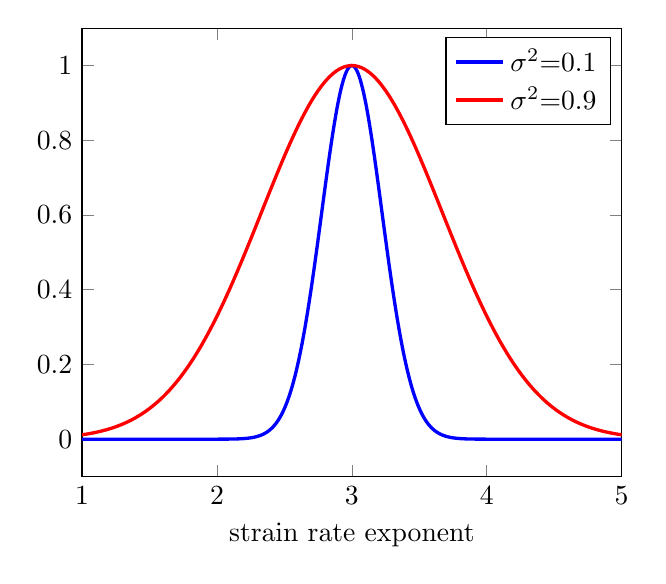
\begin{tikzpicture} 
\begin{axis}[ xlabel=strain rate exponent,xmin=1.0, xmax=5.0 ] % invoke external gnuplot as % calculator: 
  \addplot [mark=none,very thick, blue, samples=1000]{exp(-(x-3.0)^2/0.1)}; 
  \addlegendentry{$\sigma^2$=0.1}
  \addplot [mark=none,very thick, red, samples=1000]{exp(-(x-3.0)^2/0.9)}; 
  \addlegendentry{$\sigma^2$=0.9}

\end{axis} 
\end{tikzpicture}
}
\hspace{-0.2cm}\subfigure[]{

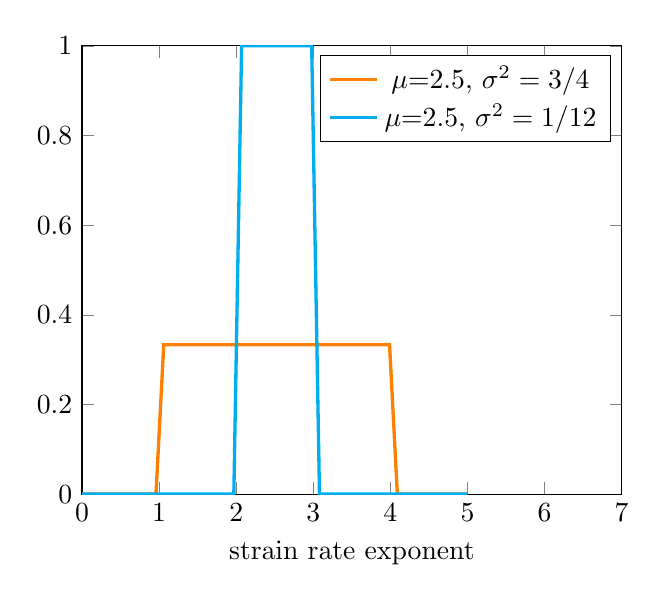
\begin{tikzpicture}[
    declare function={unipdf(\x,\xl,\xu)= (\x>\xl)*(\x<\xu)*1/(\xu-\xl);}
]
\begin{axis}[xlabel = strain rate exponent,
    samples=100,
%    const plot mark mid,
    xmin = 0, xmax = 7,
    ymin=0,ymax=1
]
\addplot [very thick, orange] {unipdf(x,1,4)};
 \addlegendentry{$\mu$=2.5, $\sigma^2 = 3/4$}
\addplot [very thick, cyan] {unipdf(x,2,3)};
 \addlegendentry{$\mu$=2.5,  $\sigma^2 = 1/12$}
\end{axis}
\end{tikzpicture}

}
%\hspace{-1.2cm}\subfigure[]{

%\begin{tikzpicture}[
%    declare function={gamma(\z)=
%    (2.506628274631*sqrt(1/\z) + 0.20888568*(1/\z)^(1.5) + 0.00870357*(1/\z)^(2.5) - (174.2106599*(1/\z)^(3.5))/25920 - (715.6423511*(1/\z)^(4.5))/1244160)*exp((-ln(1/\z)-1)*\z);},
%    declare function={gammapdf(\x,\k,\theta) = \x^(\k-1)*exp(-\x/\theta) / (\theta^\k*gamma(\k));}
%]

%\begin{axis}[
 %   axis lines=left,
%    enlargelimits=upper,
%    samples=50,
%    legend entries={$k=1\quad \theta=2$,$k=2\quad \theta=2$, $k=9\quad \theta=0.5$}
%]
%\addplot [smooth, domain=0:20] {gammapdf(x-3,1,2)};
%\addplot [smooth, domain=0:20, red] {gammapdf(x-3,2,2)};
%\addplot [smooth, domain=0:20, blue] {gammapdf(x-3,9,0.5)};
%\end{axis}
%\end{tikzpicture}
%}
\caption{(a) Normal distributions for the strain rate exponent prior (b)Uniform distributions for the strain rate exponent prior. In (a) we compare the possibility of using two different normal distributions to demonstrate our knowledge or lack thereof of what the values of the strain rate exponent should be. }
\label{fig:prior_ex} 
\end{figure}

 Another possibility for a prior distribution is using a \textit{non-informative prior}\citep{Tarantola05}. A non-informative prior give equal likelihood (equal probability) to each value such that no preference is given to a single value. Using non-informative priors can be advantageous when it is not apparent what an acceptable value is for a parameterized quantity such as the weakfactor.  An example of a non-informative prior is the uniform distribution in Fig.\ref{fig:prior_ex}b for the strain rate exponent. A uniform distribution has the following properties,
\begin{align}
\mathcal{U}(a,b) =
\begin{cases}
 \frac{1}{b-a}   &b\geq x \geq a \\
               0 &\quad \text{otherwise} \\
\end{cases}
\end{align}
with a mean and variance of 
\begin{align}
\begin{split}
\mu(a,b) &=\frac{1}{2}(a+b) \\
\sigma^2(a,b) &=\frac{1}{12}(b-a)^2 .\ \\
\end{split}
\end{align}

The uniform distribution in Fig.~\ref{fig:prior_ex}b has the same mean; however the variance is different. Compared to a normal distribution, the variance for the uniform distribution is determined by the range of likely values, each of which has the same probability.


 For a prior that is described by a normal distribution the mean $\mu$ and covariance, $\mathcal{C}$ is needed.
\begin{equation}
\ppi_{prior} = \mathcal{N}(\mu,\mathcal{C})
\end{equation}
Taking the negative log of the prior distribution results in a weighted misfit,
\begin{equation}
\mathcal{J}_{prior} = \frac{1}{2}(\mm-\mm_{mean})^T\mathcal{C}^{-1}(\mm-\mm_{mean})
\end{equation}
Therfore, the cost function would be
\begin{equation}
\begin{split}
  \mathcal{J}(\uu,\mm,p)&:= \frac{1}{2}\int_{\partial \Omega_1} (\mathcal{O}\uu-\uu_{\text{obs}})^T\mathcal{C}^{-1}_{vel}(\mathcal{O}\uu-\uu_{\text{obs}})d\partial\Omega_1 \\
%  &+\frac{1}{2}(\eta_0 - \text{exp}({\int_{\Omega_i} \ln \eta}))^{2} \\
   &+(\eta_0 - \text{exp}({\int_{\Omega_i} \ln \eta}))^{2} +\frac{1}{2}(\mm-\mm_{mean})^T\mathcal{C}^{-1}(\mm-\mm_{mean}).
\end{split}
\end{equation}
While the solution to the adjoint equation does not change, the gradient term for each parameter is modified,
\begin{equation}
\mathcal G:= \int_{\Omega} 2 \eta_{,i}(\IIinv, \Gamma, n, \sigma_y)\strain(\uu):\strain(\vv) d\Omega  + \mathcal{C}^{-1}(\mm-\mm_{mean})\mm_i.\
\end{equation}
Computing gradients, we will use these new gradients to update the parameters as they measure the sensitiviy the the parameters are to the observations.

\section*{Model Setup}
We have constructed a set of model constraints based on global observations. There are four components of these constaints: a global temperature distribution, the geometry of faults, the kinematics of plate motion, and the bounds on the effective viscosity within selected regions.

The temperature model has been constructed globally in a spherical shell from which  we have taken selected cross-sections. The temperature of the oceanic lithosphere follows a half-space cooling model using  updates to the digital grid of the age of the oceanic plates \citep{muller1997digital}. The thermal structure of slabs were constructed as follows: initially the top surface of the slabs was based on the Slabs 1.0 surface with normals pointing downward with the initial thermal structure of slabs based on the half space model using the age of the plate at the position of the trench. Then we solved for thermal conduction at each depth computed transiently over a duration equal to the travel time to reach the depth with the local convergence velocity (using the relative velocity vector). Although solved only with conduction, this procedure resulted in thermal structures close to those obtained in fully dynamic models.

\begin{figure}[H]
\centering
\scalebox{0.5}{
\hspace{-1.8cm}\subfigure[]{
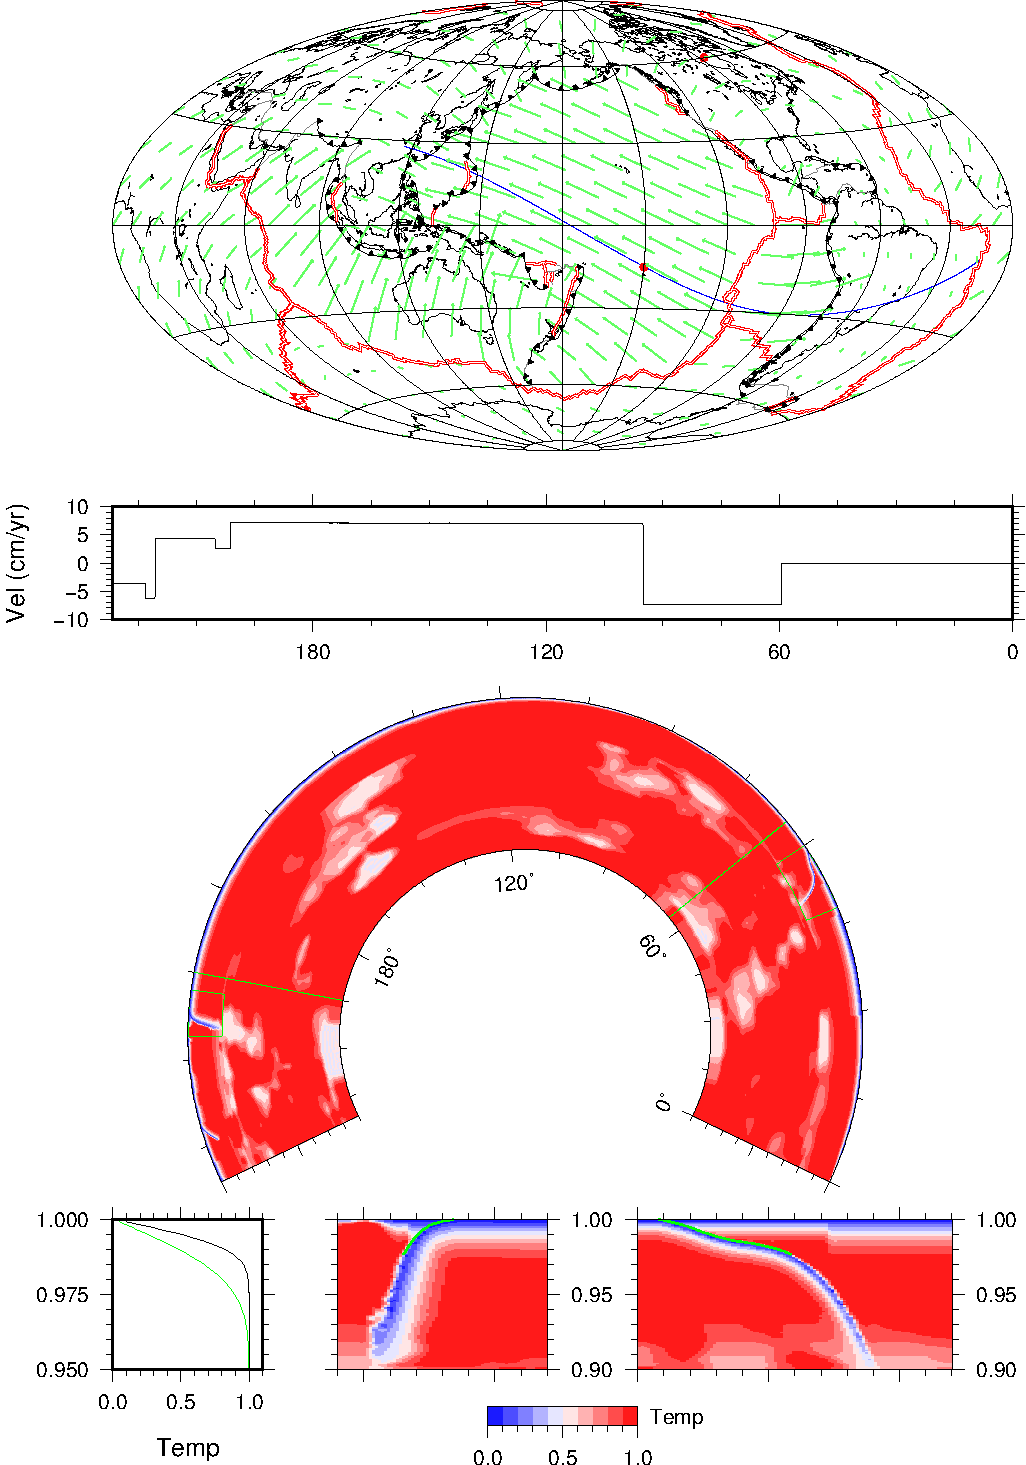
\includegraphics[height=150mm,width=100mm]{slab_temp.pdf}%{mesh.pdf}
}

\hspace{-1.cm}\subfigure[]{
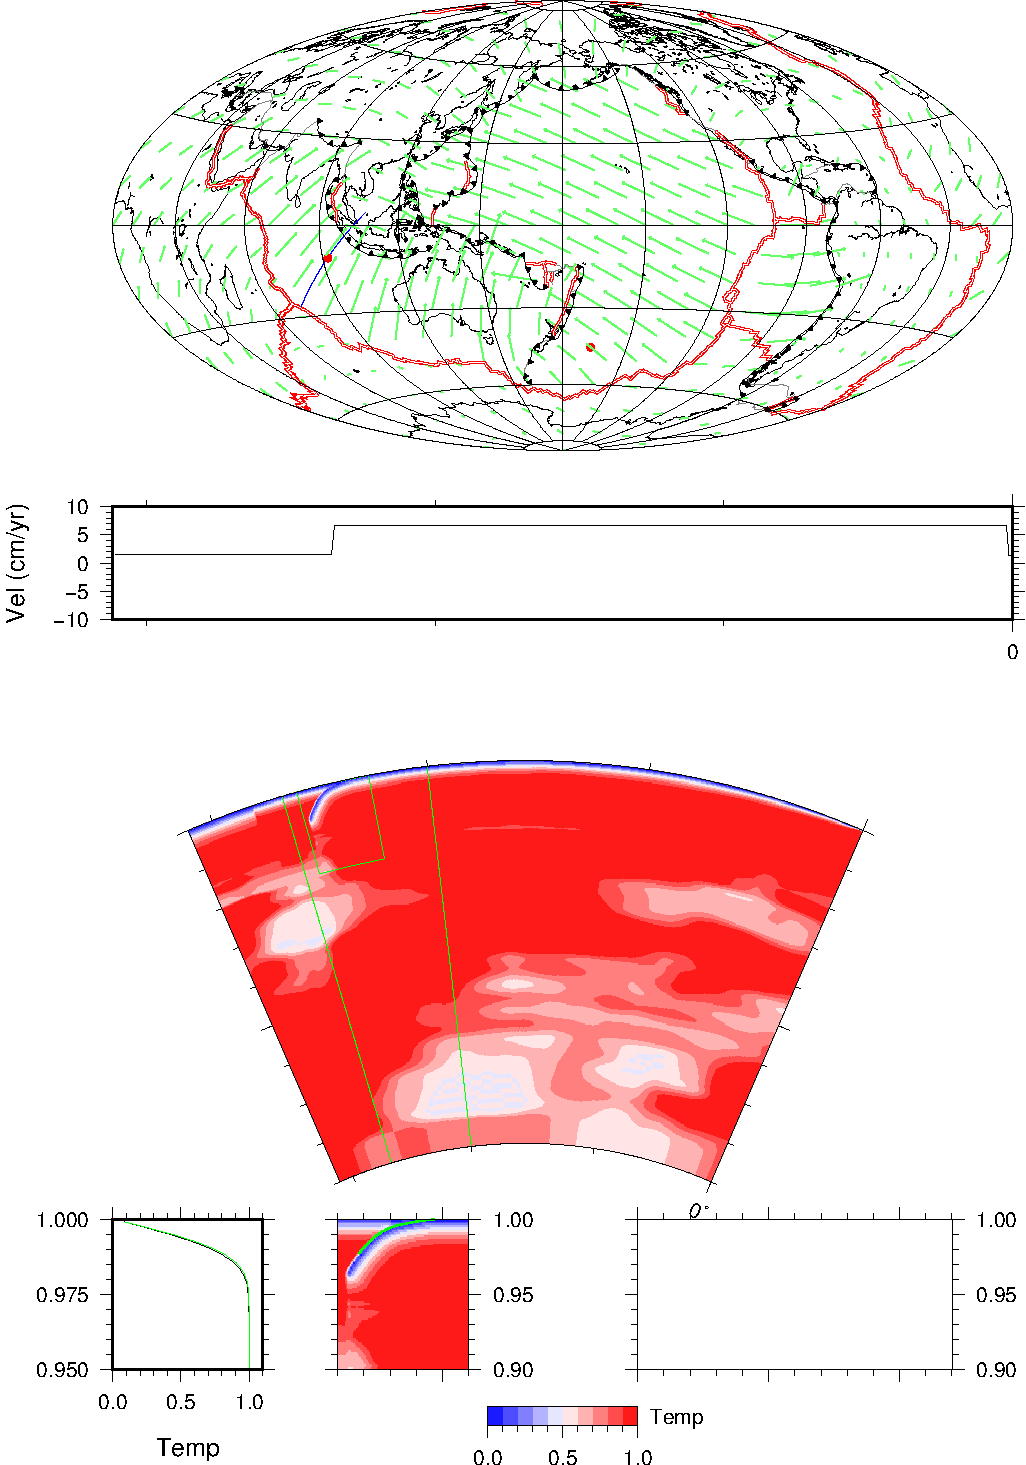
\includegraphics[height=150mm,width=100mm]{slab_temp_sumatra.pdf}%{mesh.pdf}
}
\scalebox{0.85}{
\hspace{-0.6cm}\subfigure[]{
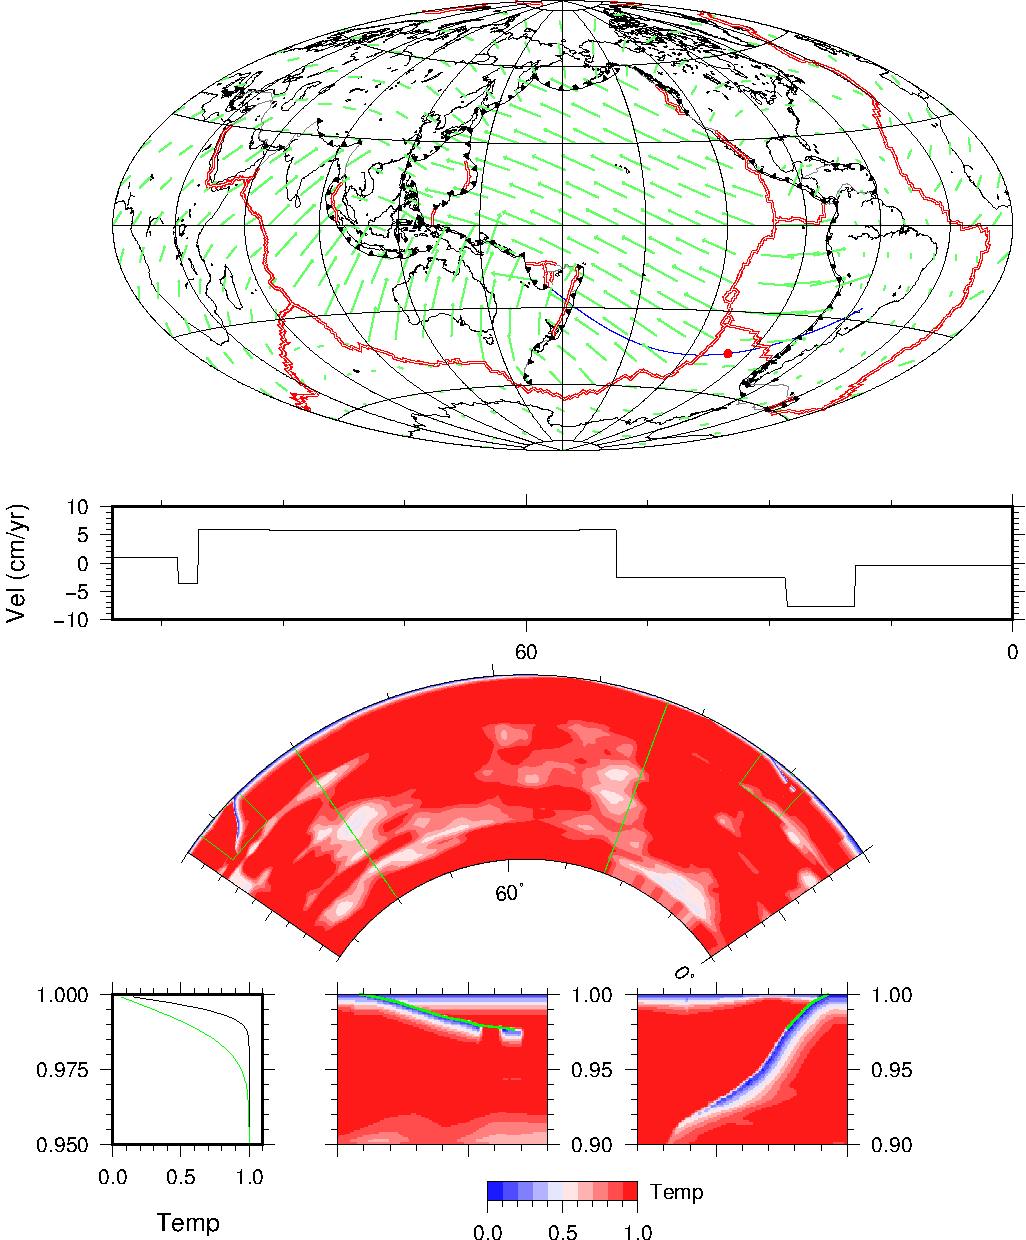
\includegraphics[height=150mm,width=100mm]{slab_temp_tonga.pdf}%{mesh.pdf}
}
}
}
\caption{(a)Cross-section used (b)input temperature distributions used with large scale thermal structures in the lower mantle (c)similar input temperature structure, except reduced large scale thermal anomalies.}
\label{fig:xsection2sumatra}
\end{figure}

These cross-sections are important as they represent the end-member cases of what is considered least to most seismically coupled. Sumatra experienced a great earthquake in 2005, while the Chilean subduction zone is known to have great earthquakes. Furthermore, there have been studies in which seismic coupling, including geodetic, have shown that there are variations in seismic coupling for subduction zones. To investigate the coupling for various seismically coupled subduction zones, we consider three cross-sections in Fig.\ref{fig:xsection2sumatra}. The cross-section in Fig.\ref{fig:xsection2sumatra}a is the larger of the three cross-sections and contains three subduction zones that are very coupled (Nazca-South America) to least coupled (Ryukyu and Izu-Bonin), which in a certain sense mimics a global model in that it represents a small portion of the variability in coupled subduction zones. The cross-sections in Fig.\ref{fig:xsection2sumatra}b,c are smaller than in  Fig.\ref{fig:xsection2sumatra}a, and thus do not contain the coupling variability of the larger cross-section; however those cross-sections represent other subduction zones that exhibit substantial coupling (Sumatra) and very little coupling (Tonga).

\begin{table}[H]
  \caption{Physical quantities used in our tests.} % title of Table
  \centering  % used for centering table
  \begin{tabular}{c c c} % centered columns (2 columns)
    \hline \hline                        %inserts double horizontal lines
    Subduction Zone & $\chi_s$ & $\chi_g$  \\ [0.5ex] % inserts table
    %heading
    \hline                  % inserts single horizontal line
    North Tonga  &0.65 &N/A   \\
    Central Peru &0.8 &0.75 \\
    South Peru &0.75 &N/A \\
    Central Chile &0.70 &1.0 \\
    South Chile  &0.82-1.0 &0.96 \\
    North Chile &0.94 &1.0 \\
    Sumatra &0.5-0.83 &1.0 \\
    \hline %inserts single line
  \end{tabular}
  \label{table:parameters} % is used to refer this table in the text
\end{table}


The decoupling of fault zones between converging plates at subduction zones, genrally thought to be the places on which great earthquakes occur, were represented as weakzones. The weakzone factors were created by a stencil with a center line of defined by the Slabs 1.0 surface \citep{Hayes2012}. The stencil was defined as
\begin{equation}
\Gamma_{stencil} = 1.0 - (1-\Gamma_i)\exp\{-(d_i-d_0)^2/(2\sigma_{smooth}^2)\}
\end{equation}
and with coefficient $\Gamma$ that was recovered in ~\eqref{eq:rheo}, $d_0$ is the center-line profile, $\sigma_{smooth}$ is the amount of smoothing for the weak zone.

On the surface of the earth we generated a veloctiy field from MORVEL56 \citep{GGGE2060}. in different reference frames. For each cross-sectional model which we generally define as great circle arcs, with local unit vector \textbf{d} in the directon of the circle, we extracted the velocity $v_{xs}=\textbf{d}\cdot\textbf{v}$. Compared to previous studies, we use an alternate form of the Arrenhius relationship, 
\begin{equation}
\eta_{thermal} = A_i\exp\{E_a(1.0-T)\} .\
\end{equation}
This change (from 0.5 to 1) is important because when the non-dimensional temperate is $1.0$, the activation energy does not change the effective viscosity (in the lower mantle), such that the effective viscosity in the lower mantle for multiple models would be the same . For our models, we assume the values of certain physical parameters of the mantle which are summarized in Table ~\ref{table:parameters}.

\begin{table}[H]
  \caption{Physical quantities used in our tests.} % title of Table
  \centering  % used for centering table
  \begin{tabular}{c c c} % centered columns (2 columns)
    \hline \hline                        %inserts double horizontal lines
    Symbol & Parameter & Value  \\ [0.5ex] % inserts table
    %heading
    \hline                  % inserts single horizontal line
    $\rho$ & Density ($\rho$)  & 3300 kg/m$^3$ \\
    $g$ & Gravity ($g$) & 9.81 m/s$^2$ \\
    $\alpha$ & Coefficient of Thermal expansion ($\alpha$) & 2 $\times$ $10^{-5}$ \\ 
    $\Delta T$& Temperature Difference $\Delta T$ & 1400 K \\
    $D$& Depth of layer ($D$) & 1500 km \\
    $\kappa$& Thermal Diffusivity ($\kappa$) & $10^{-6}$  m$^2$/s \\
    $\eta_{\text{ref}}$& Reference Viscosity  ($\eta_{\text{ref}}$) & $10^{20}$ Pa $\cdot$ s \\
    Ra & Rayleigh Number (Ra) & 2.92 $\times$ $10^9$ \\
    $n$ & Strain rate exponent in upper/lower mantle ($n$) & 3.0/1.0 \\
    \hline %inserts single line
  \end{tabular}
  \label{table:parameters} % is used to refer this table in the text
\end{table}


While the tomography in the lower mantle such as the SR40 or \citep{simmons2012llnl}, there is also a non-uniqueness in reference frames. For example, we will look at how the parameter inferences vary depending on what surface velocity models are used. Furthermore, for the surface velocity data in Fig.\ref{fig:xsection2}, we keep the left most plate fixed as its velocity is almost $0$cm/year. We therefore present multiple case studies where we explore the effect of different lower mantle structure, types of observed data used.

 The plate motion data is highly dependent on the reference frame used such as hotspots, one fixed to a specific plate (Pacific for example), or the no-net-rotation(NNR) reference frame. From plate motion models, we have the Euler pole (latitude and longitude) of each plate along with the rotation (degrees/Ma), where there is uncertainty of both pole and the rotation. Furthermore, each global plate motion model is non-unique in the sense of plate motion velocity and uncertainty, which can possibly influence the parameter estimation of plate couplings. Using various plate motion models can 
 
 There are particular issues with the surface velocity data. It is known that from the large lateral variations in viscosity produces net-rotation of the lithosphere which in turn would mean that the NNR velocities would be incorrect.  We will make use of these different pieces of plate velocities data to determine what if any effect plate motion models have on the inference of plate boundary couplings. 

\begin{figure}[H]
\centering
\hspace{-0.85cm}\subfigure{
  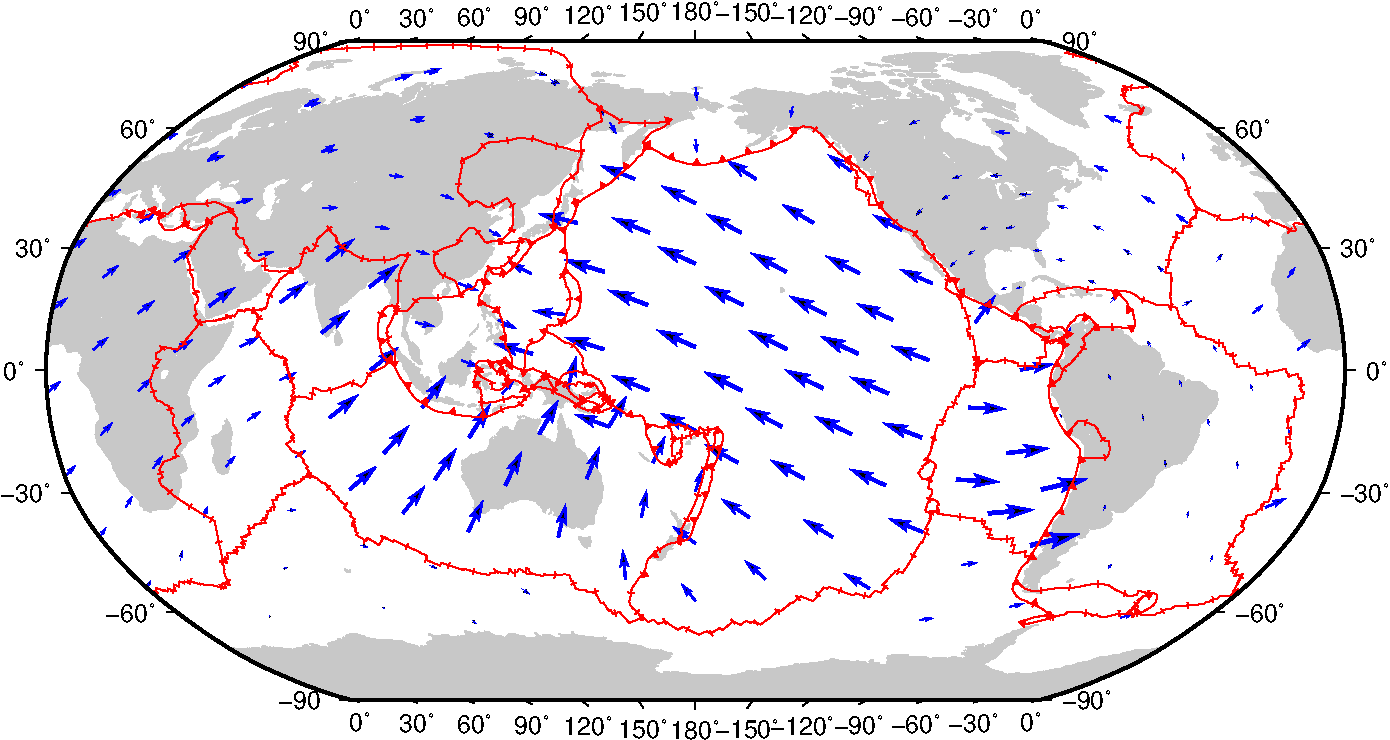
\includegraphics[height=60mm,width=128mm]{morvel2.pdf}%{mesh.pdf}
}
\caption{Plate velocities with error ellipses from NNR-MORVEL56}
\label{fig:platevel}
\end{figure}


As presented earlier, the average effective viscosity data is an additional constraint that we will explore to determine the effect it has on the inference of the the rheological parameters. It is posited that since the effective viscosity is an observation from the mantle, then this data should better constraint on the global parameters such as the strain rate exponent, activation energy, and upper mantle prefactors. We will place the average effective viscosity constraint under the South American plate. 

\section*{Results}
\subsection*{Inversions}
We will infer multiple parameters from the cross-sectional model to ascertain the coupling of subduction zones and the inferred global parameters such as the yield stress and strain rate exponent. However, to explore both the strengths and limitations of the optimization, we initially focus on a single section shown in Fig.\ref{fig:xsection2sumatra}a.  %This cross-section has the advantage of a great circle that is nearly tangent to plate velocity vectors for the fast moving plates. We exploit this profile, almost  25,410km in length as it implies the laws occur a spheical center; one of the most seismically coupled zones, Chile and one of the least seismically coupled Marianas, while also having one margins with  back-arc extension. 

To infer the couplings and global parameters, we need to have an initial guess for the rheological parameters  for the forward model. In all models, we choose an initial guess for weakzone factor of $\Gamma=10^{-5}$, which typically decouples the plate boundaries such that subduction occurs. We choose an initial guess of 125 MPa for the yield stress because it provides a reasonable amount of dynamic weakening in forward models while satisfying estimates from seismicity \citep{craig2014reassessment}. The strain rate exponent of $n=3.0$ is a value that is associated with the mantle and within the bounds imposed from laboratory experiments and an activation energy $E_a=17.5$ such that plates are strong enough to act as stress guides. %We set up a reference case with 
%the strain rate exponent, yield stress and plate boundary couplings, and the upper mantle prefactor as unknowns.  
Choosing the initial guess of the activation energy is important such that a small activation energy can give rise to a large yield stress \citep{crameri2017dynamical} which does not satisfy bounds from seismicity. Furthermore, we choose to infer the radial prefactor of the upper mantle, a parameter that controls the effective viscosity of the upper mantle.  


%We use this cross-section as the surface velcoities are almost-parallel the the great-circle. The length of this arc is approximately, 25,410 km.
For the cross-sectional model in Fig.\ref{fig:xsection2sumatra}a, we ran a suite of inversions where we varied which parameters will be inferred in Table \ref{table:inversions}.  We first inferred the plate couplings, strain rate exponent, yield stress and upper mantle prefactor as shown in Case 1 and Fig.\ref{fig:inverse1}. The effective viscosity in Case 1 (Fig.\ref{fig:inverse1}a) shows a weak upper mantle in addition to dynamic weakening in hinge zones.  In Case 1, we were able to infer the plate couplings within 5 adjoint iterations (Fig.\ref{fig:inverse1}c), which is similar to what as observed in \citep{ratnaswamy2015adjoint}. Furthermore, the inferred strain rate exponent is slightly greater than 3.0 (initial guess), while the inferred yield stress is 148 MPa, which is larger than the initial guess of 125 MPa. Similar to our previous studies \citep{ratnaswamy2015adjoint}, we find that there is an inference of different plate couplings regardless of the starting initial guess. The relative ordering of inferred plate couplings in Case 1 strongly suggests that the inferred coupling may lend credence to the notion that the Nazca-South America plate boundary is more coupled compared to Ryukyu and Izu-Bonin plate margins. A new parameter that is included in the inversion for Case 1 is the upper mantle prefactor,  which may not clearly have physical meaning compared to the strain rate exponent and yield stress, but plays an important part in controlling the effective viscosity in the upper mantle and to a degree, the amount of shear thinning in the upper mantle. 


\begin{sidewaystable}
\centering
	\begin{table}[H]
		\caption{Case study summary} % title of Table
		\centering  % used for centering table
		\begin{tabular}{c c c c c c c  } % centered columns (2 columns)
		\hline \hline                        %inserts double horizontal lines
		Case & Subduction Zone &n. &$\sigma_y$&Weakfactor (SAM/RYU/IZU/SUM/TON) $x10^{-5}$ &UM Prefactor &Viscosity data   \\ [0.5ex] % inserts table
		%heading
		\hline                  % inserts single horizontal line
	        1 &Complete& 3.042 & 148 & $100/0.82/0.77/NA/NA$ &  4700& no \\
	        2 &Complete& 3.046 & 146 & $67.3/0.773/0.798/NA/NA$ & no & no \\
	        3 &Complete& 3.0225 & 141.8 & $87.3/0.703/0.7448/NA/NA$ & no & yes \\
	        4 &Complete& 3.08 & 155 & $94.6/0.8423/0.889/NA/NA$ & no & no (priors used) \\
             5 &Sumatra& N/A & N/A & N/A &  4700& no \\
	        6 &Sumatra& N/A & N/A & N/A & no & no \\
	        7 &Sumatra& N/A & N/A & N/A & no & yes \\
	        8 &Sumatra& N/A & N/A & N/A & no & no (priors used) \\
             9 &Tonga& N/A & N/A & N/A &  4700& no \\
	        10 &Tonga& N/A & N/A & N/A & no & no \\
	        11 &Tonga& N/A & N/A & N/A & no & yes \\
	        12 &Tonga& N/A & N/A & N/A & no & no (priors used) \\
                
                \hline %inserts single line
		\end{tabular}
		\label{table:inversions} % is used to refer this table in the text
		\end{table}
\end{sidewaystable}

 In case 2, we now only infer the plate couplings, yield stress and strain rate exponent, which was similarly done in \citep{ratnaswamy2015adjoint}, with plate motion data (80 \% of plate coverage). In this case, we find that the inferred strain rate exponent is 3.042, which is close to the initial guess of 3.0, (similar to Case 1) and is only 0.13\% larger than the inferred strain rate exponent in Case 1. Similar to the strain rate exponent, the inferred yield stress in Case 2 is 146 MPa, only 1.35\% lower than the inferred yield stress in Case 1. The inferred plate couplings in Case 2 also follow the same pattern as the least coupled subduction zones are Ryukyu and Izu-Bonin. 

In case 3, we now infer the plate couplings, yield stress and strain rate exponent; however, we include the average effective viscosity below South America. In this case, we find that the strain rate exponent is 3.0225, which is smaller than the inferred strain rate exponent in Cases 1 and 2. The inferred yield stress for Case 3 is 141.8 MPa which is quite similar to the inferred yield stress from Cases 1 and 2. Similar to Cases 1 and 2, we find that there is a preferred coupling for each subduction zone, such that the Nazca-South America subduction zone is the most coupled, (approximately an order of magnitude more), compared to Izu-Bonin and Ryukyu subduction zones. %Furthermore, the inferred strain rate exponent in Case 2 is only 0.13\% larger than the inferred strain rate exponent in Case 1. Similar to the strain rate exponent, the inferred yield stress in Case 2 is 146 MPa, only 1.35\% lower than the inferred yield stress in Case 1. The inferred plate couplings in Case 2 also follow the same pattern as the least coupled subduction zones are Ryukyu and Izu-Bonin. 

In case 4, we similarly infer the plate couplings and global rheological parameters; however, we use prior information for the yield stress, strain rate exponent and plate couplings. For the plate couplings, we impose a prior with mean of $10^{-5}$, strain rate exponent of 2.95 and yield stress of 120 MPa. In this case, we wanted to test how well we can infer the rheological parameters using apriori information for the inferred parameters. With prior knowledge, we find that the order of plate couplings corresponds to what was found from cases 1-3. Furthermore, the recovered strain rate exponent is approximately the same (3.08), while the yield stress is slightly larger (155 MPa), than cases 1-3. 

 % The first case study is shown below in Fig.\ref{fig:inverse1}
\begin{figure}[H]
\centering
\hspace{-0.2cm}\subfigure[]{
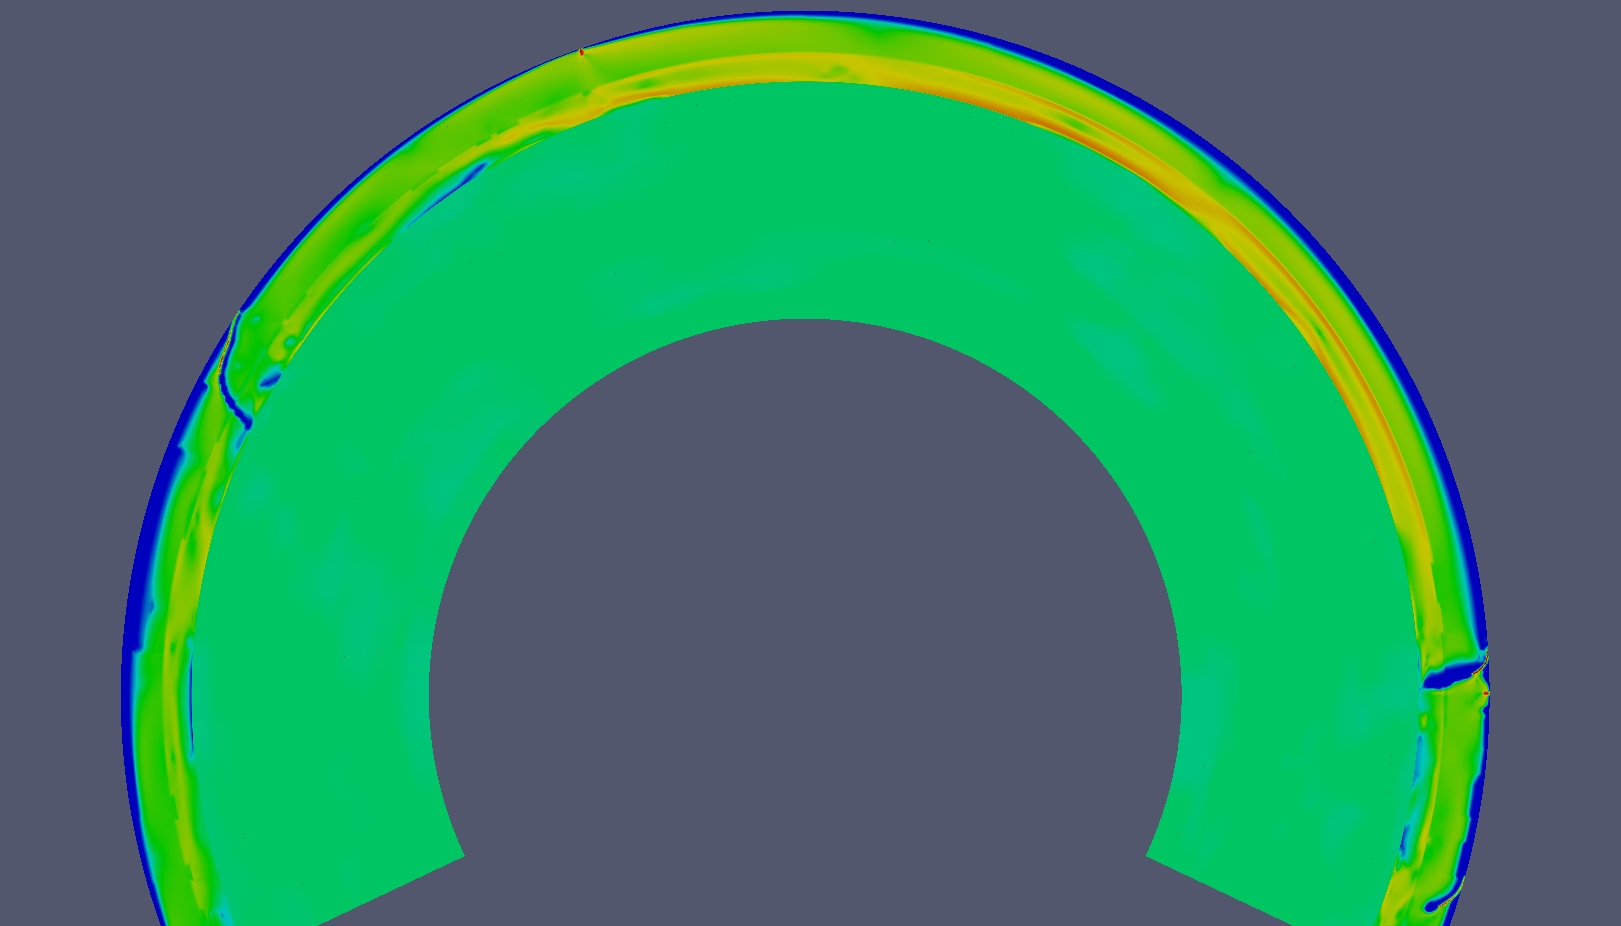
\includegraphics[height=65mm,width=128mm]{visc_no_stress.jpg}%{mesh.pdf}
}
\hspace{-0.85cm}\subfigure[]{
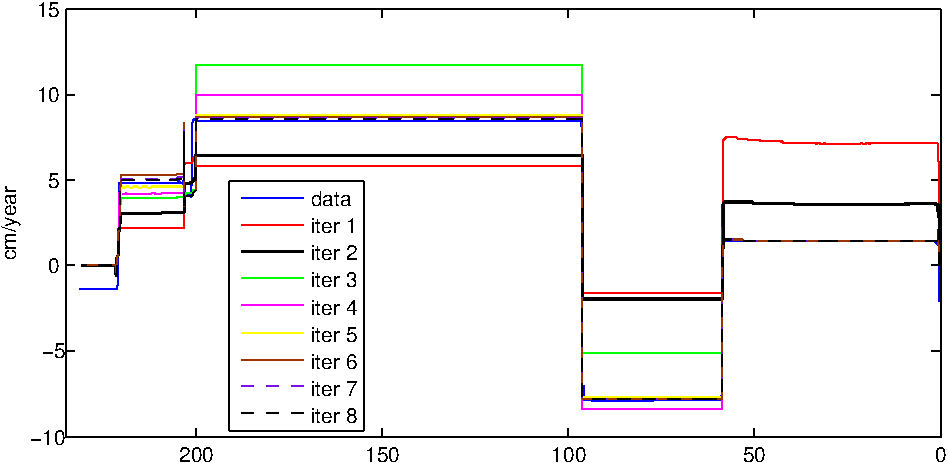
\includegraphics[height=35mm,width=68mm]{datavel2.pdf}%{mesh.pdf}
}
\hspace{-0.2cm}\subfigure[]{
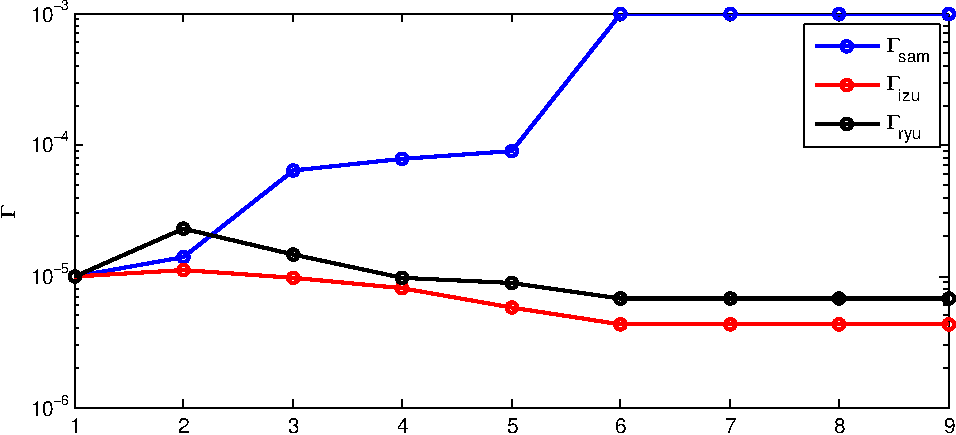
\includegraphics[height=35mm,width=58mm]{gammainv2.pdf}%{mesh.pdf}
}
\hspace{-0.2cm}\subfigure[]{
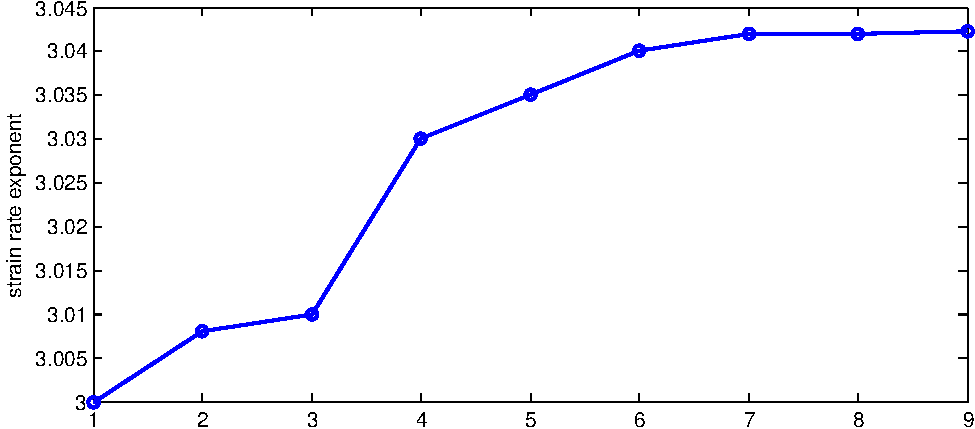
\includegraphics[height=35mm,width=58mm]{strainexpinv2.pdf}%{mesh.pdf}
}
\hspace{-0.2cm}\subfigure[]{
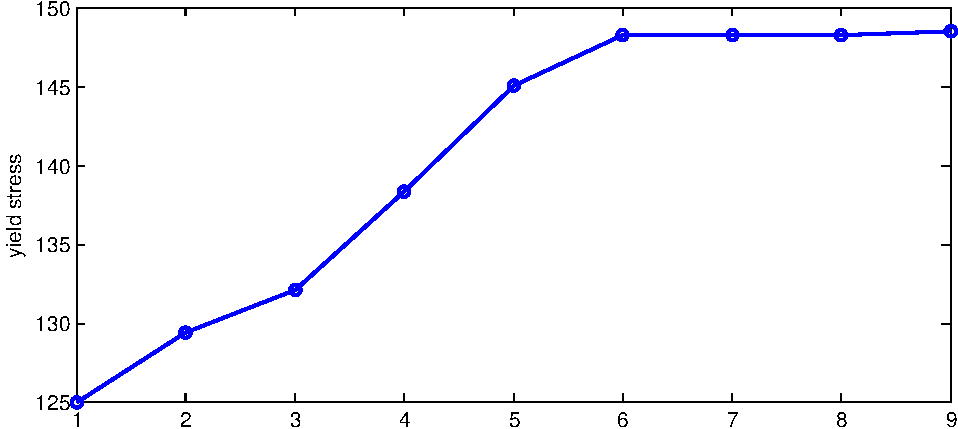
\includegraphics[height=35mm,width=58mm]{yieldstressinv2.pdf}%{mesh.pdf}
}
\hspace{-0.2cm}\subfigure[]{
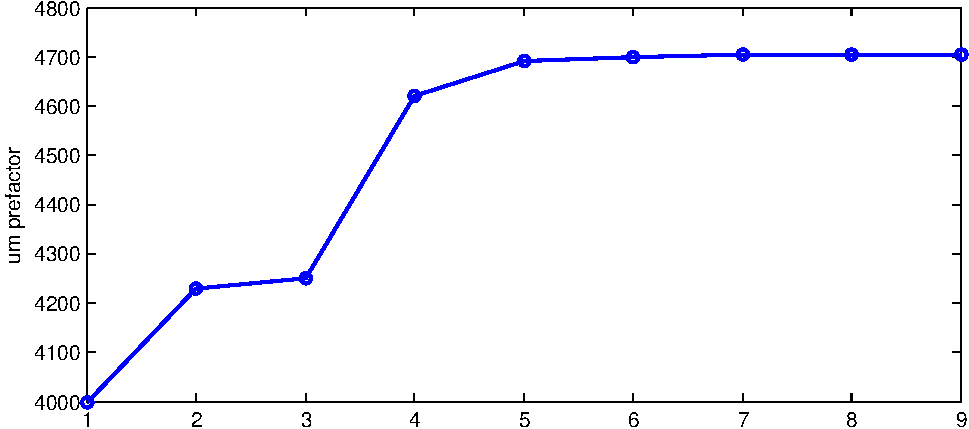
\includegraphics[height=35mm,width=58mm]{uminv2.pdf}%{mesh.pdf}
}
\caption{(a) Effective viscosity structure (b)Surface velocity comparison between data and different iterations.(c)Plate boundary weakfactor iteration (d) strain rate exponent iteration (e) yield stress iteration (f) upper mantle prefactor iteration.}
\label{fig:inverse1}
\end{figure}

%\begin{figure}[H]
%\centering
%\hspace{-0.2cm}\subfigure[]{
%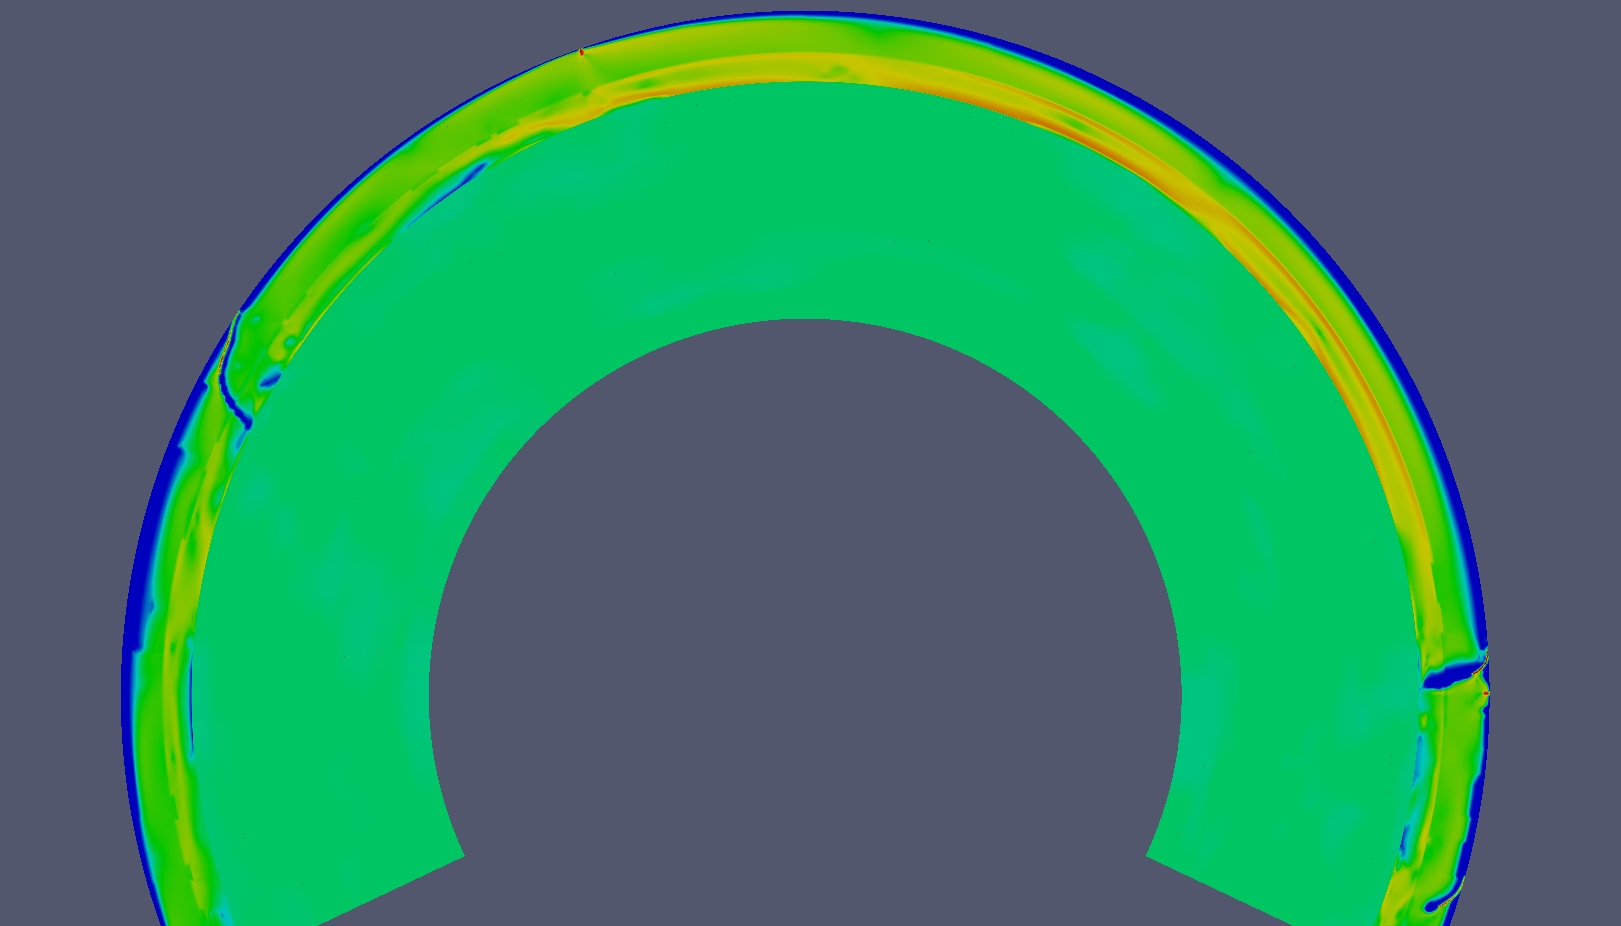
\includegraphics[height=65mm,width=128mm]{visc_no_stress.jpg}%{mesh.pdf}
%}
%\caption{Effective viscosity structure}
%\end{figure}

%For the inversion, we look at the the conditional distributions for the global rheological parameters are shown in Fig.\ref{fig:strain_cond} for the strain rate exponent, yield stress and upper mantle prefactor. In previous studies, we did not not look at the upper mantle prefactor and its contribution in the statistical sense.
%\begin{figure}[H]
%\centering
%\hspace{-0.85cm}\subfigure[]{
%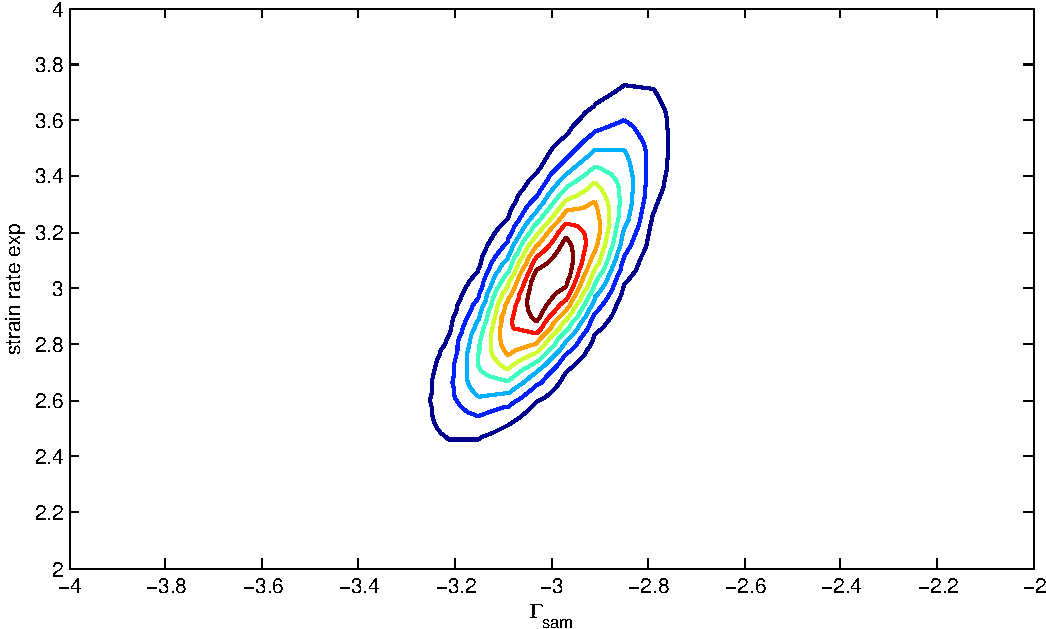
\includegraphics[height=35mm,width=68mm]{strain_sam.pdf}%{mesh.pdf}
%}
%\hspace{-0.2cm}\subfigure[]{
%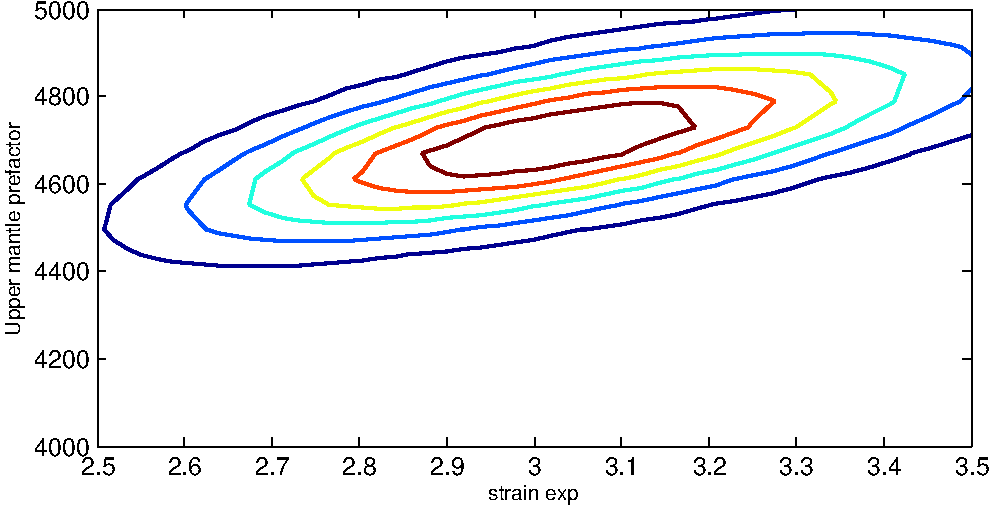
\includegraphics[height=35mm,width=58mm]{n_up.pdf}%{mesh.pdf}
%}
%\hspace{-0.2cm}\subfigure[]{
%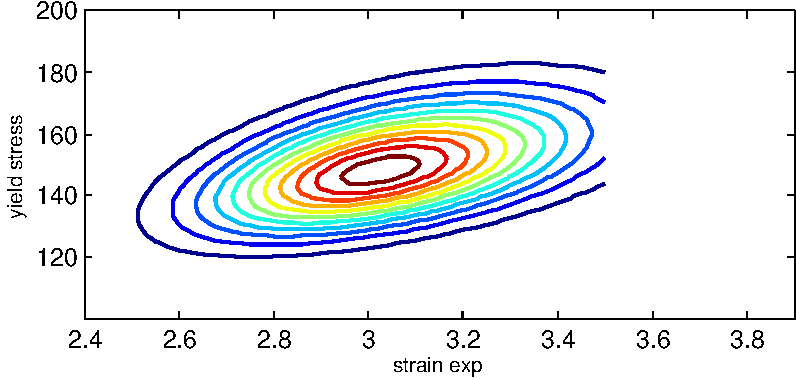
\includegraphics[height=35mm,width=58mm]{n_yield.pdf}%{mesh.pdf}
%}
%\caption{(a)Conditional distributions for Strain rate exponent-South America weakfactor (b) Conditional distributions for Strain rate exponent-upper mantle prefactor (c)Conditional distributions for Strain rate exponent-yield stress}
%\label{fig:strain_cond}
%\end{figure}
%From the conditional distribution of the strain rate exponent vs the weakfactor of South America plate boundary, there exists a positive correlation. Additionally, for the strain rate exponent vs. the yield stress and upper mantle prefactor, there also exists a positive correlation.


% An important study is how these parameters are influenced based on the thermal anomalies in the lower mantle. To investigate this, we remove the tomographic features from the lower mantle by setting the activation energy to be zero. Doing so effectively, makes the lower mantle homogeneous in effective viscosity (i.e. no thermally activated viscosity).
%In the first case study (the reference case), we infer the strain rate exponent , the yield stress, and the plate boundary prefactors. There are three subduction zones, 

%THe resulting inversions are shown below in Fig.\ref{fig:refcase}.
%\begin{figure}[H]
%\centering
%\hspace{-0.2cm}\subfigure[]{
%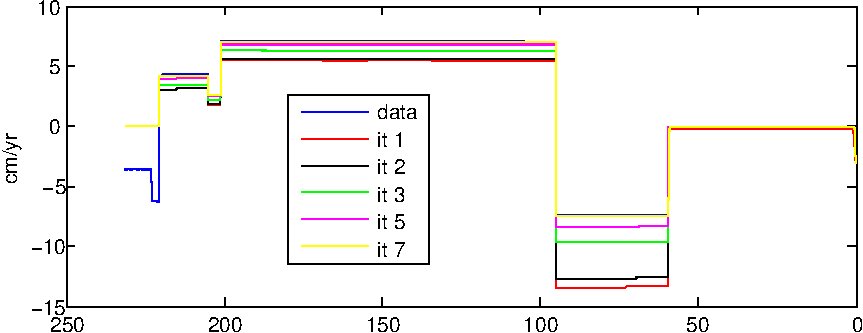
\includegraphics[height=35mm,width=58mm]{data_no_stress.pdf}%{mesh.pdf}
%}
%\hspace{-0.2cm}\subfigure[]{
%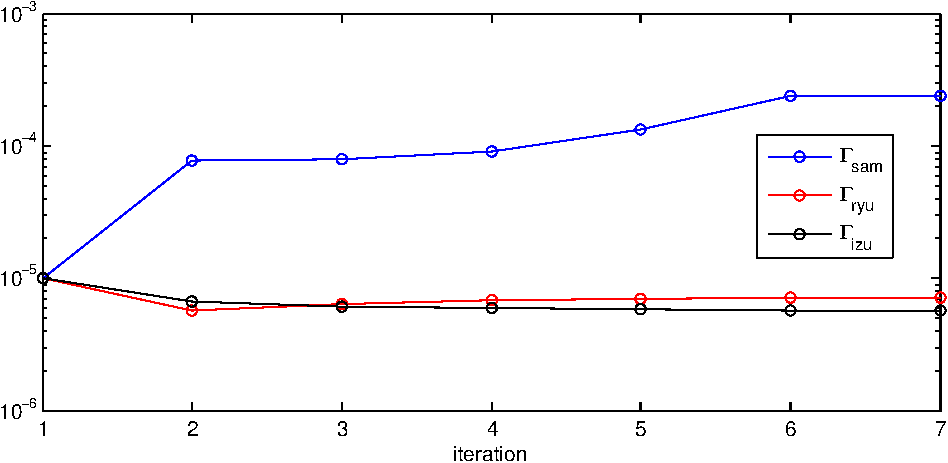
\includegraphics[height=35mm,width=58mm]{gamma_stress_guide.pdf}%{mesh.pdf}
%}
%\hspace{-0.2cm}\subfigure[]{
%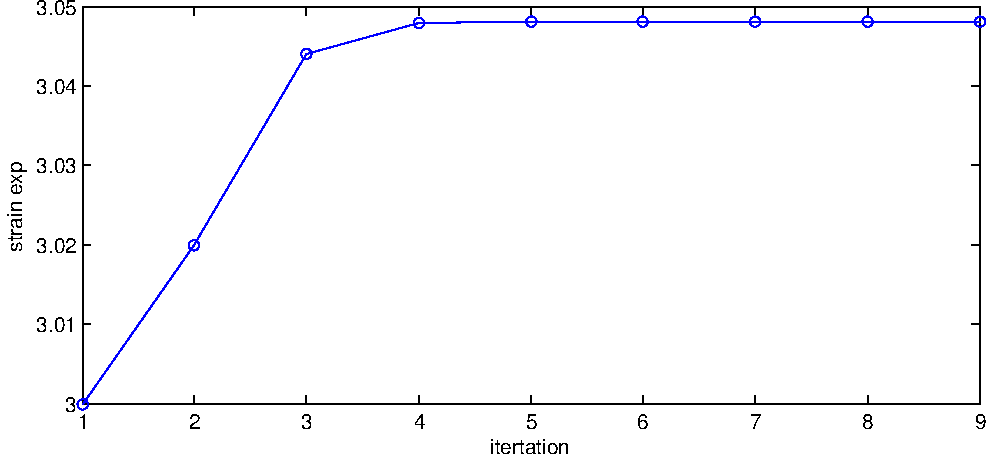
\includegraphics[height=35mm,width=58mm]{stain_exp_stress_guide.pdf}%{mesh.pdf}
%}
%\hspace{-0.2cm}\subfigure[]{
%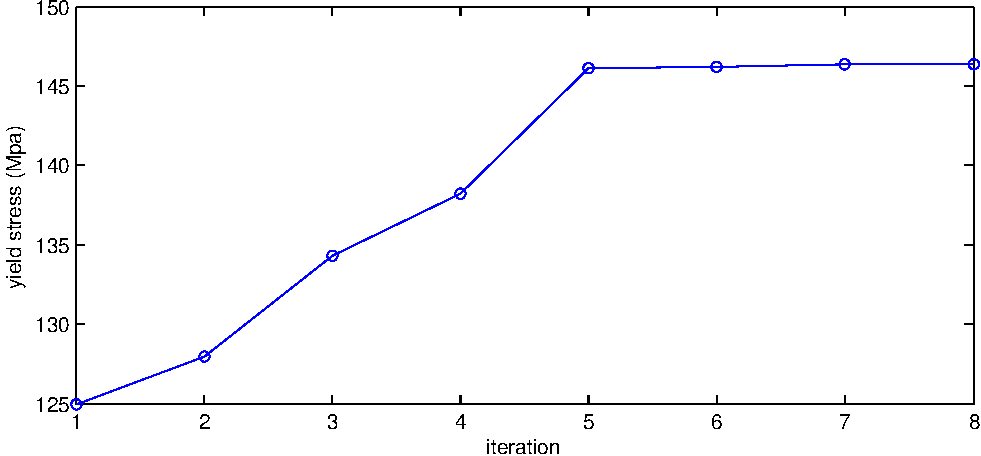
\includegraphics[height=35mm,width=58mm]{yield_stress_guide.pdf}%{mesh.pdf}
%}
%\caption{(a)Surface velocity comparison between data and different iterations.(b)Plate boundary weakfactor %iteration (c) strain rate exponent iteration (d) yield stress iteration (e) upper mantle prefactor iteration}
%\label{fig:refcase}
%\end{figure}

%For the case study in Fig.\ref{fig:refcase}, we inferred the weakzone prefactors, strain rate exponent, and yield stress for the 2D cross-section. In this model , we see that we are able to minimize the misfit in plate motions for each iteration. Compared to our previous work \citep{ratnaswamy2015adjoint}, where we know the inferred parameters, in these cases we do not know them. Furthermore, we note that this inversion is stable in that for each iteration, there does not seem to be any fluctuations in the inferred values.  When inferring the global parameters, in a least-squares optimization problem we obtain a point estimate, the \textbf{MAP} point. However, to better ascertain the correlations between the parameters, we look at the conditional distribuitions between the parameters.

%\begin{figure}[H]
%\centering
%\hspace{-0.85cm}\subfigure[]{
%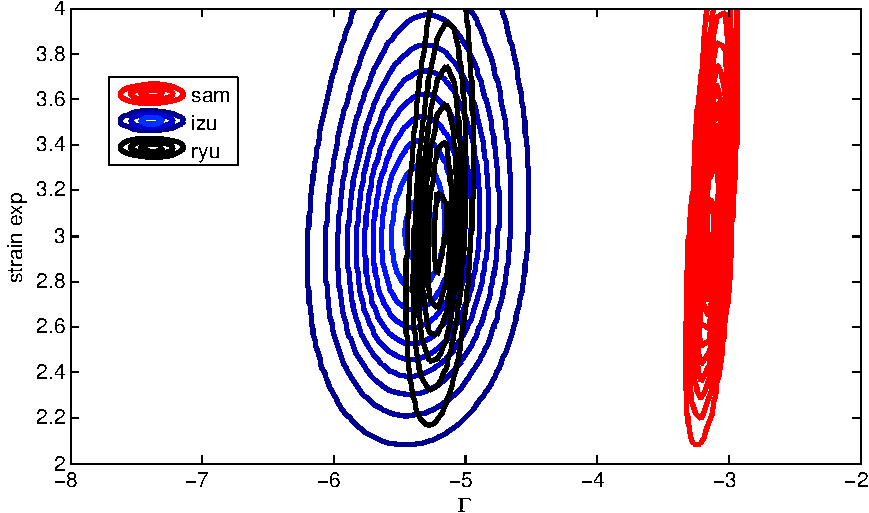
\includegraphics[height=35mm,width=68mm]{gauss_weak_strain.pdf}%{mesh.pdf}
%}
%\caption{(a)Conditional distributions for Izu-Ryukyu weakfactor (b)Conditional distributions for Izu-South America weakfactor (c)Conditional distributions for South America-Ryukyu weakfactor.}
%\end{figure}



%In the figure below, the conditional distributions for each weakfactors are shown.
%\begin{figure}[H]
%\centering
%\hspace{-0.85cm}\subfigure[]{
%\includegraphics[height=35mm,width=68mm]{izu_ryu.pdf}%{mesh.pdf}
%}
%\hspace{-0.2cm}\subfigure[]{
%\includegraphics[height=35mm,width=58mm]{izu_sam.pdf}%{mesh.pdf}
%}
%\hspace{-0.2cm}\subfigure[]{
%\includegraphics[height=35mm,width=58mm]{ryu_sam.pdf}%{mesh.pdf}
%}
%\caption{(a)Conditional distributions for Izu-Ryukyu weakfactor (b)Conditional distributions for Izu-South America weakfactor (c)Conditional distributions for South America-Ryukyu weakfactor.}
%\end{figure}
%We can see that there are not as strong correlations between the weakfactor space of South American and Izu-Bonin (and Ryukyu). This maybe attributed to the plate boundaries not being connected to each other which would therefore decrease the influence of one plate on the other.

% The conditional distributions for the strain rate exponent with respect to the weakfactors are shown in Fig.\ref{fig:strain_cond}.


%As outlined earlier, there are certain places where we have estimates of the average effective rheology in the mantle. We now invert for the rheological parameters with an average area of viscosity beneath the South America plate as well as plate motions . The results are shown in the figure below. %One can see that the inferred parameters converge to a stationary value.
%\begin{figure}[H]
%\centering
%\hspace{-0.2cm}\subfigure[]{
%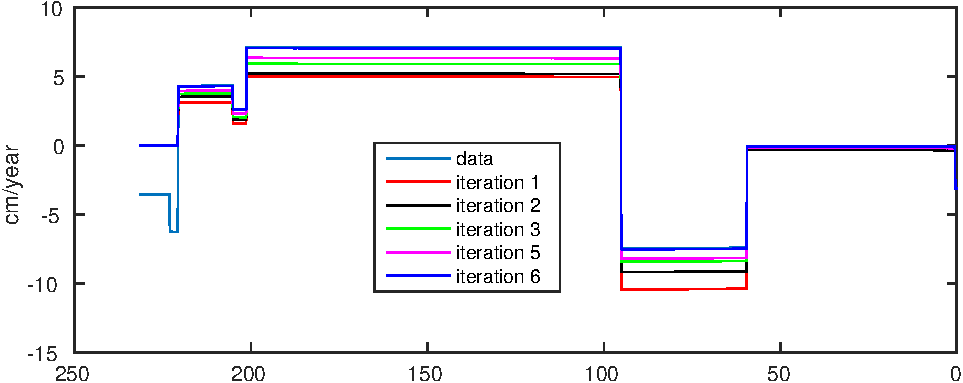
\includegraphics[height=35mm,width=58mm]{inv2data.pdf}%{mesh.pdf}
%}
%\hspace{-0.2cm}\subfigure[]{
%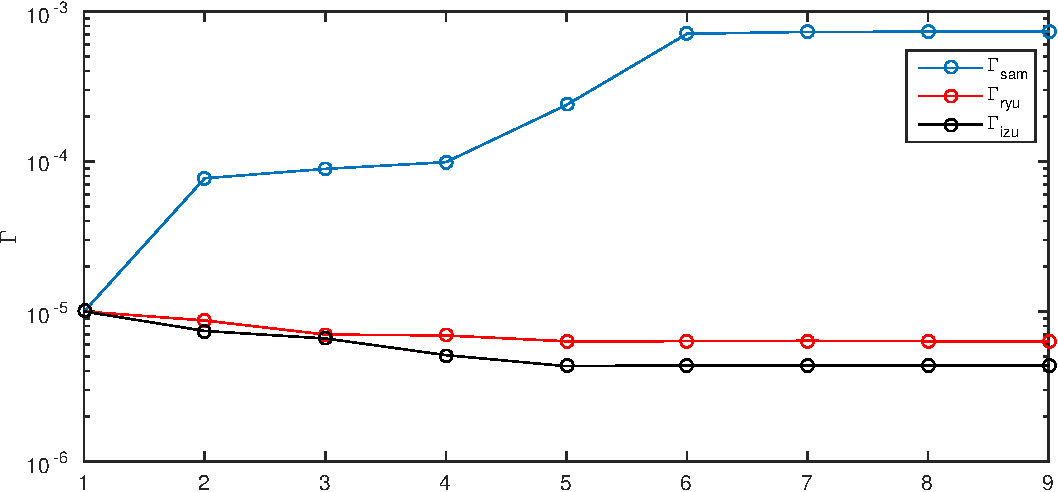
\includegraphics[height=35mm,width=58mm]{prefactordata2.pdf}%{mesh.pdf}
%}
%\hspace{-0.2cm}\subfigure[]{
%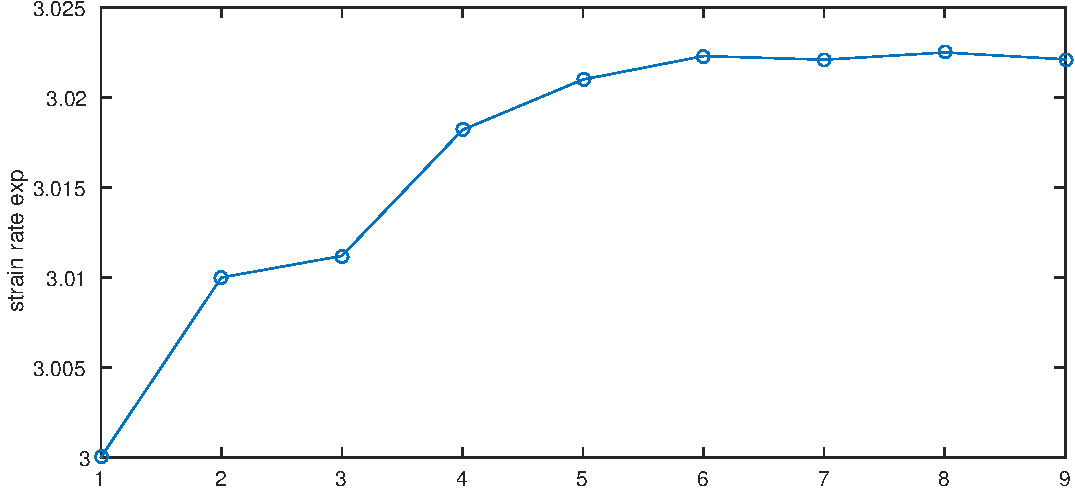
\includegraphics[height=35mm,width=58mm]{strainexpdata2.pdf}%{mesh.pdf}
%}
%\hspace{-0.2cm}\subfigure[]{
%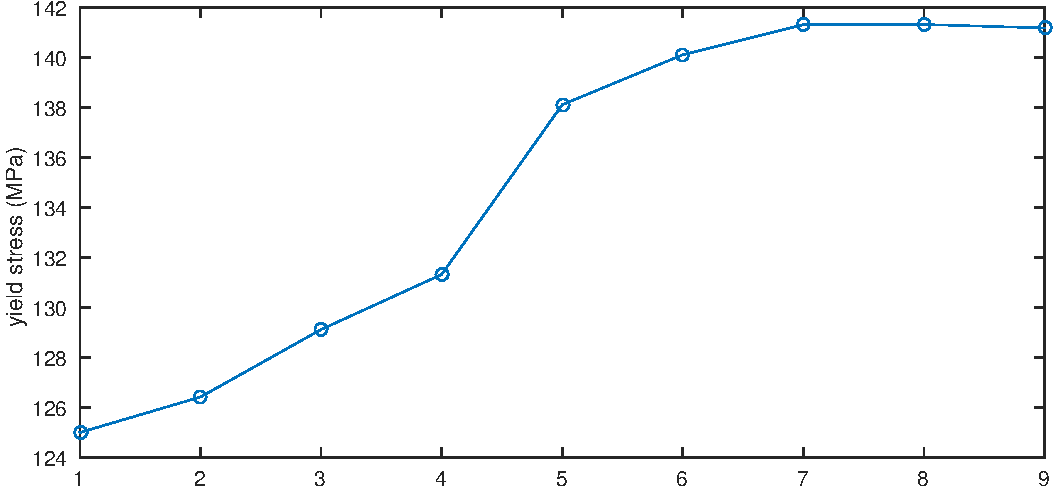
\includegraphics[height=35mm,width=58mm]{yieldstressdata2.pdf}%{mesh.pdf}
%}
%\caption{(a)Surface velocity comparison between data and different iterations.(b)Plate boundary weakfactor iteration (c) strain rate exponent iteration (d) yield stress iteration}
%\end{figure} 
%As in the reference case, the inferred values are stable and converge to stationary values. Furthermore, the conditional distributions are shown below for select plate boundary weakfactors vs. global quantities. 
%\begin{figure}[H]
%\centering
%\hspace{-0.85cm}\subfigure[]{
%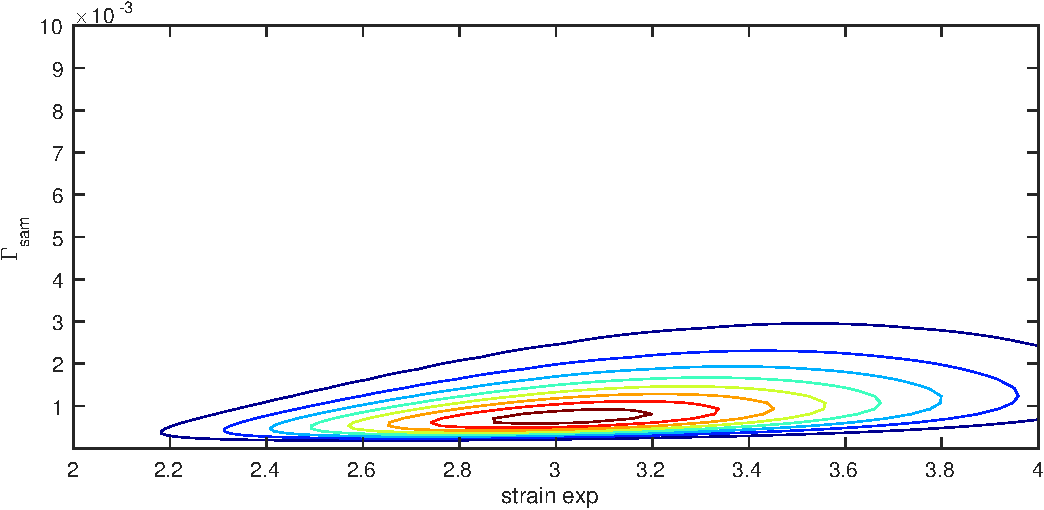
\includegraphics[height=45mm,width=58mm]{gauss_strain.pdf}%{mesh.pdf}
%}
%\hspace{-0.2cm}\subfigure[]{
%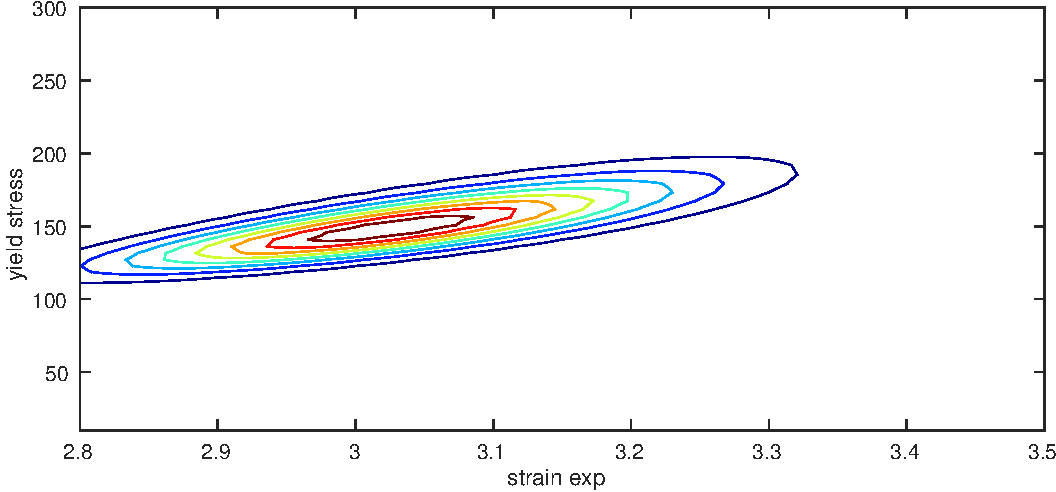
\includegraphics[height=45mm,width=58mm]{gauss_yield.pdf}%{mesh.pdf}
%}
%\caption{(a)Conditional distributions for Strain rate exponent-South America weakfactor (b)Conditional distributions for Strain rate exponent-yield stress}
%\label{fig:global}
%\end{figure}
%while the plate boundary conditionals are shown in the figure below.
%\begin{figure}[H]
%\centering 
%\hspace{-0.2cm}\subfigure[]{
%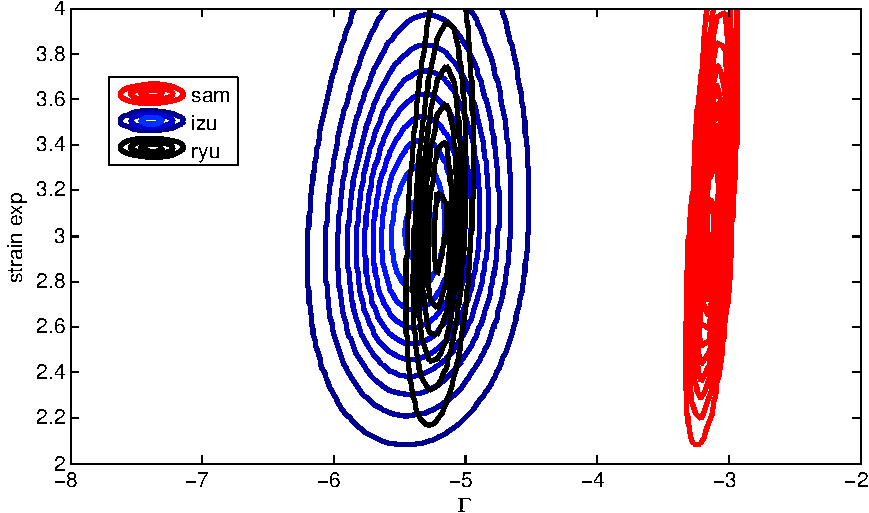
\includegraphics[height=35mm,width=58mm]{gauss_weak_strain.pdf}%{mesh.pdf}
%}
%\hspace{-0.2cm}\subfigure[]{
%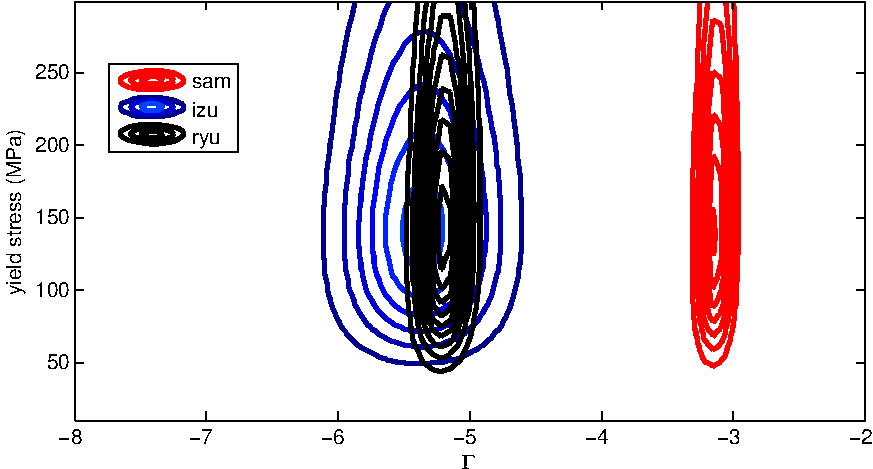
\includegraphics[height=35mm,width=58mm]{gauss_weak_yield.pdf}%{mesh.pdf}
%
%\hspace{-0.2cm}\subfigure[]{
%\includegraphics[height=35mm,width=58mm]{ryu_sam2.pdf}%{mesh.pdf}
%}
%\caption{(a)Conditional distributions for Izu-South America(b)Conditional distributions for Izu-Ryukyu (c)Conditional distributions for Ryukyu-South America weakfactor}
%\end{figure}
 
%\section*{Inversions with Priors}
%In the previous inversions, we did not make use of prior knowledge of the global parameters. However, there have been experimental studies in which there are bounds on certain parameters such as the strain rate exponent. Here, we test what parameters we infer when we add prior knowledge for the weakfactors, yield stress and strain rate exponent. In this case study, we invert for the strain rate exponent, yield stress and plate boundary couplings. The initial guess for the 
%plate boundary couplings is $\Gamma = 10^{-5}, n=3.0, \sigma_y = 125$MPa. We assumed Gaussian priors and the subsequent inversions are shown below,
%\begin{figure}[H]
%\centering
%\hspace{-0.2cm}\subfigure[]{
%\includegraphics[height=35mm,width=58mm]{weakfactor_prior.pdf}%{mesh.pdf}
%}
%\hspace{-0.2cm}\subfigure[]{
%\includegraphics[height=35mm,width=58mm]{yield_stress_prior.pdf}%{mesh.pdf}
%}
%\hspace{-0.2cm}\subfigure[]{
%\includegraphics[height=35mm,width=58mm]{strain_exp_prior.pdf}%{mesh.pdf}
%}
%\caption{(a)Weakfactor prior (b) yield stress prior (c) strain rate exponent prior.}
%\end{figure}

%The resulting inversion is shown in the figure below. One can see that with relatively weak priors we are able to infer the yield stress, strain rate exponent, and corresponding weakfactors. 
%\begin{figure}[H]
%\centering
%\hspace{-0.2cm}\subfigure[]{
%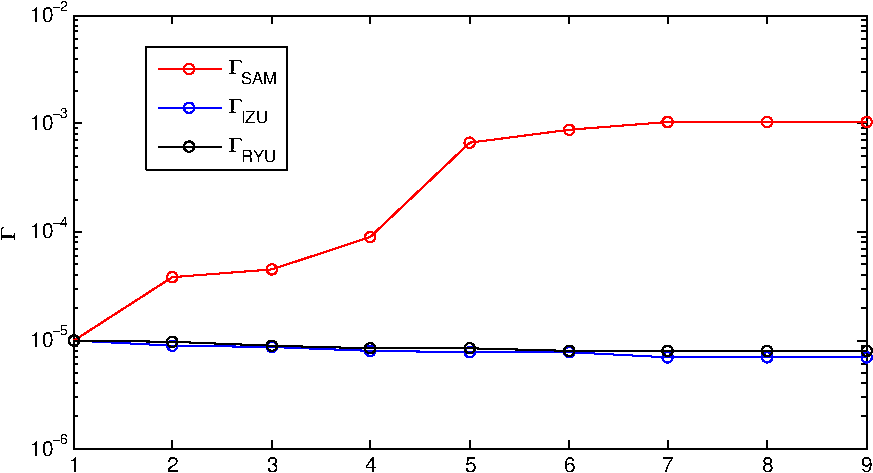
\includegraphics[height=35mm,width=58mm]{prefactor_prior_inv.pdf}%{mesh.pdf}
%}
%\hspace{-0.2cm}\subfigure[]{
%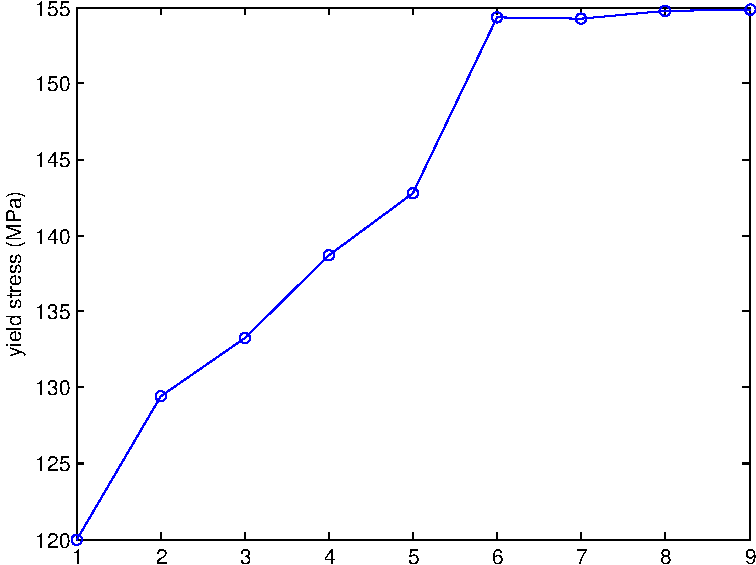
\includegraphics[height=35mm,width=58mm]{yield_stress_prior_inv2.pdf}%{mesh.pdf}
%}
%\hspace{-0.2cm}\subfigure[]{
%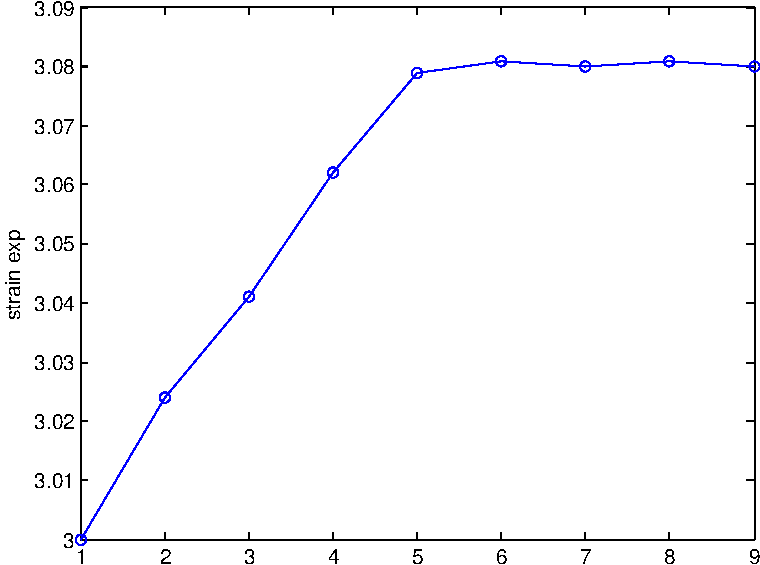
\includegraphics[height=35mm,width=58mm]{strain_exp_prior_inv2.pdf}%{mesh.pdf}
%}
%\caption{(a)Plate boundary weakfactor iteration (b) yield stress iteration (c) strain rate exponent iteration}
%\end{figure}

%The distributions of the stresses within each plate boundary is shown below.

\subsection*{Uncertainty Quantification for Plate boundary stresses}


An important part of our studies was to quantify the uncertainty of the inferred rheological parameters that was similarly done in \citep{ratnaswamy2015adjoint} by examining the posterior distributions, more specifically the conditional distributions. In Fig.\ref{fig:distrib}a,b, we compare the conditional distributions for the plate couplings vs yield stress and strain rate exponent in Case 1 and find that there is a clear demarcation between the least coupled subduction zones (Ryukyu and Izu-Bonin) and South America. We find that the South America plate boundary is more coupled compared to Ryukyu and Izu-Bonin regardless of the global parameter (yield stress and strain rate exponent).
 Additionally, we find that there still exist strong positive correlations between the strain rate exponent and yield stress, and a negative correlation between the plate couplings and strain rate exponent that were previously observed in \citep{ratnaswamy2015adjoint}.  The upper mantle prefactor is another parameter that we inferred, and we find that there is a positive correlation between the upper-mantle prefactor and strain rate exponent, i.e. an increase in strain rate exponent yields an increase in the upper mantle prefactor. 

\begin{figure}[H]
\centering
\hspace{-0.2cm}\subfigure[]{
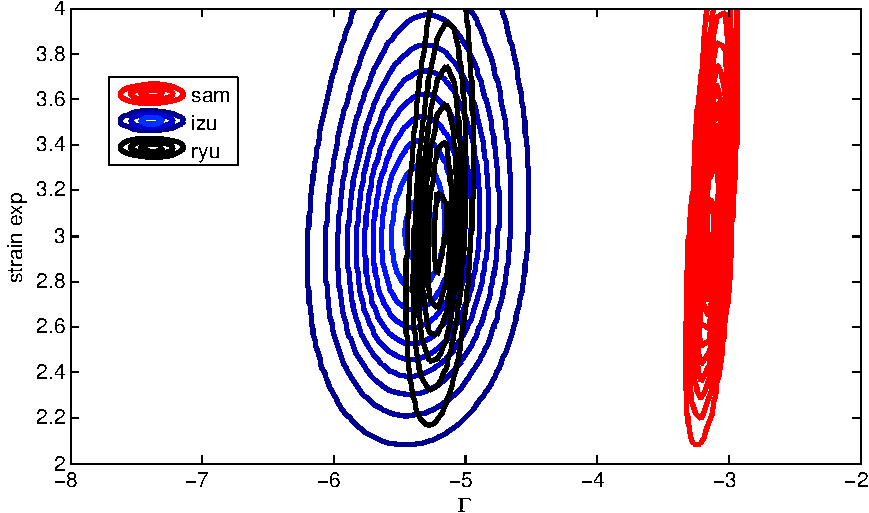
\includegraphics[height=35mm,width=58mm]{gauss_weak_strain.pdf}%{mesh.pdf}
}
\hspace{-0.2cm}\subfigure[]{
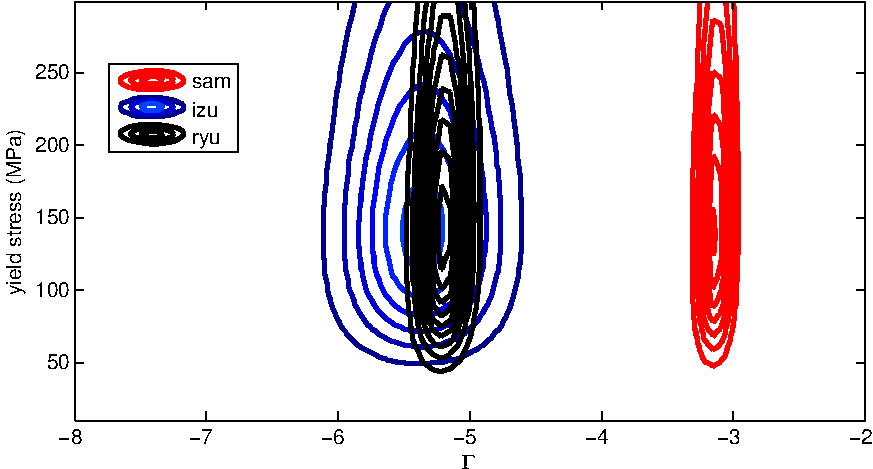
\includegraphics[height=35mm,width=58mm]{gauss_weak_yield.pdf}%{mesh.pdf}
}
\hspace{-0.2cm}\subfigure[]{
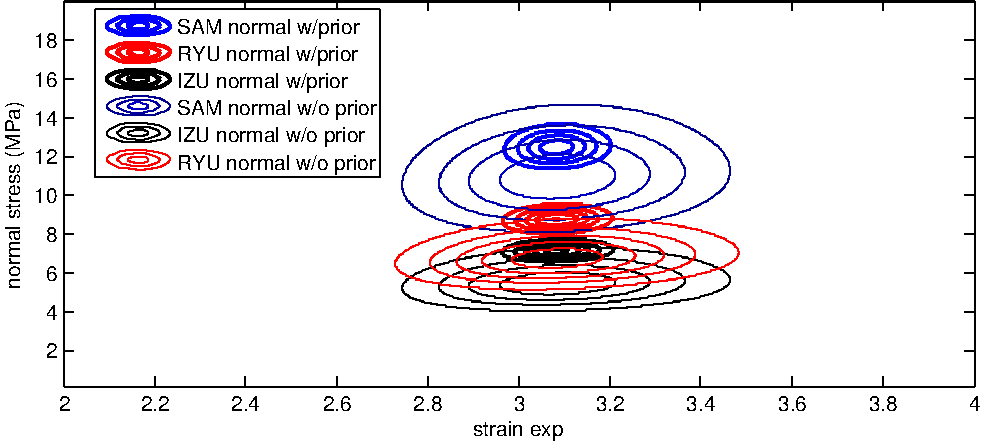
\includegraphics[height=35mm,width=58mm]{normal_comparison_prior2.pdf}%{mesh.pdf}
}
\hspace{-0.2cm}\subfigure[]{
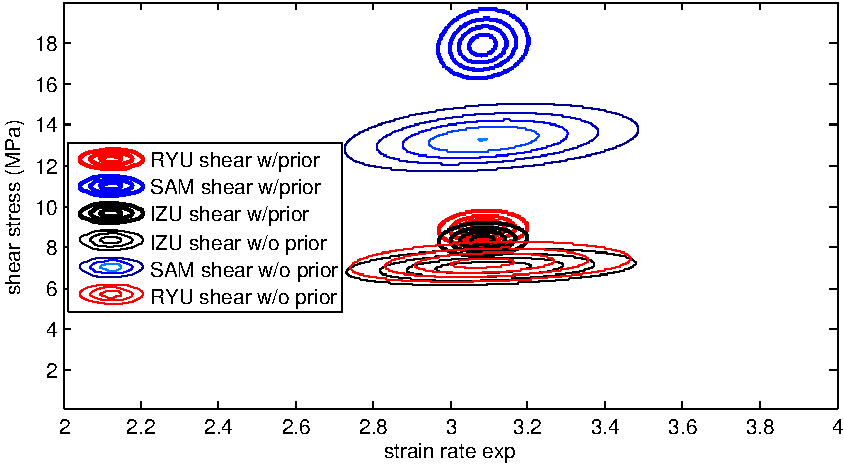
\includegraphics[height=35mm,width=58mm]{shear_comparison_prior.pdf}%{mesh.pdf}
}
\caption{(a)Strain rate exponent vs plate coupling (b) Yield stress vs plate coupling (c) Normal  stress vs. strain rate exponent (d)Shear  stress vs. strain rate exponent}
\label{fig:distrib}
\end{figure}


In Case 2, we have find that the conditional distributions were similar to those in \citep{ratnaswamy2015adjoint}, which is not surprising as we inferred the same parameters, (strain rate exponent, yield stress, and plate couplings). In case 3, we included additional (average viscosity) data to infer those same parameters as in Case 2. We found similarly that there exists correlations between the strain rate exponent, yield stress and plate couplings that were found in Case 2. However, we found that for the global parameters such as the strain rate exponent had less uncertainty, i.e. the variance is smaller.

In Case 4, we  used priors for the plate couplings, yield stress and strain rate exponent.We found that the \textbf{MAP} point did not change as much compared to the \textbf{MAP} points from Cases 1-3; however, each of the parameters' uncertainty has been reduced as similar to \citep{ratnaswamy2015adjoint}.


\begin{table}[H]
  \caption{Mean normal and shear stress for each subduction zone.} % title of Table
  \centering  % used for centering table
  \begin{tabular}{c c c c c c} % centered columns (2 columns)
    \hline \hline                        %inserts double horizontal lines
    Case & South America & Izu-Bonin & Ryukyu & Sumatra & Tonga   \\ [0.5ex] % inserts table
    %heading
    \hline                  % inserts single horizontal line
    1 & N/A  & N/A &N/A & N/A & N/A \\
    2 &  N/A  & N/A &N/A & N/A & N/A \\
    3 &  N/A  & N/A &N/A & N/A & N/A \\
    4 &  N/A  & N/A &N/A & N/A & N/A \\
    5 &  N/A  & N/A &N/A & N/A & N/A \\
    6 &  N/A  & N/A &N/A & N/A & N/A \\
   7 & N/A  & N/A &N/A & N/A & N/A \\
    \hline %inserts single line
  \end{tabular}
  \label{table:parameters} % is used to refer this table in the text
\end{table}


One of the key analyses that was developed in this chapter was the characterization of the uncertainty of the stresses (shear and normal) of each plate boundary that is built upon a Gaussian approximation around the \textbf{MAP} point for each inversion from Cases 1 to 4. We  In Fig.\ref{fig:distrib}c, we compare the mean normal stresses of each plate boundary and find that there is a similar pattern of the partitioning between the least coupled subduction zones of Ryukyu and Izu-Bonin to the more coupled subduction zone.

We similarly find in Fig.\ref{fig:distrib}d that the shear stresses (case 1) also have a similar trend for the partitioning of the normal stress for the more coupled plate boundary of South America compared to least coupled (Izu-Bonin and Ryukyu). However, we note that the mean of the computed normal stress is lower than the shear stresses, which is certainly not expected. Furthermore, we note that in the cases of both the shear and normal stresses, there seems to be an indication that plate coupling (both prefactor and stresses) seem to be independent of the rheology of the mantle.

%\vrnote{Need to do runs with priors without stress-guide}

\section*{Discussion}
In our case studies, we explored multiple parameter spaces than was previously done. The case are of geophysical importance as they represent the variations in seismic coupling  In the reference case we added the upper mantle prefactor to the inference space and were able to infer those parameters. In that case study, the inversion is stable in the sense that there are no large fluctuations for each inferred parameter. Furthermore, we see that the misfit in the observed plate motions is minimized in the presented inversions. %It is important to note this as  we do not know the true values of the inferred parameters with using this data.

 For the reference case, we also look at the conditional distributions such as the strain rate exponent and yield stress vs. the upper mantle prefactor. These distributions suggest that there are correlations between these global parameters. As was seen before in \citep{ratnaswamy2015adjoint}, there is a positive correlation between the yield stress and strain rate exponent. Furthermore, we see that there is a positive correlation between the upper mantle prefactor and the strain rate exponent.

We also looked at the inference of the plate motions without the upper mantle prefactor data in Fig\ref{fig:inverse1}. As was the case with the upper mantle prefactor, the inversion is stable and we are able to ascertain what rheological parameters should be to minimize plate motion data. We look at how the plate couplings would vary according to the global parameters. In Fig.\ref{fig:global} there seems to be an Independence between the plate boundary prefactors and the global quantities. This outcome suggests that the plate boundary couplings is independent of the strain rate exponent.

As pointed out, we also did inversions with effective viscosity data. From these inversions, we inferred the plate couplings, yield stress and strain rate exponent. We find that there is a slightly different value of the yield stress and strain rate exponent. However, what remains is that there there is a difference in the coupling strength of each plate boundary. The most coupled and least coupled still remains the South America-Nazca plate boundary, while the Marianas and Ryukyu are less coupled.

An important avenue we explored was the inferences of the shear and normal stresses. We see that the cumulative normal and shear stress distributions within each plate boundaries show there is a larger normal and shear stress for South America compared to the Marianas and Ryukyu subduction zones. Furthermore, we note that these plate couplings seem to be independent of the global rheological parameters such as the strain rate exponent and yield stress. When using prior information, we also find similar trends in the coupling behavior. Furthermore, we see that with this additional knowledge the conditional distribution is smaller.

%\section*{Conclusion}

\bibliography{references}


\end{document}

